\documentclass[a4paper,12pt]{article}
\usepackage{../styledoc19}


\begin{document} % конец преамбулы, начало документа
	
	\itsHSE
	\academicTeacher{Преподаватель департамента \vfill программной инженерии  факультета компьютерных наук}
	{М. К. Горденко}
	
	\projectName{IOS-ПРИЛОЖЕНИЕ <<СОЦИАЛЬНАЯ СЕТЬ ДЛЯ СОТРУДНИКОВ НИУ ВШЭ>>}
	
	\titleList{Программа и методика испытаний}{RU.17701729.04.03-01 51 01-1}
	\par\vspace{60mm}
	\nameOfAuthor{БПИ174}{Д. Ю. Редникина}
	\tabForFirstPage
	
						\newpage
	
	\pagestyle{fancy}
	\lhead{УТВЕРЖДЕН \newline
	 	RU.17701729.04.03-01 51 01-1}
	\vspace*{\fill}
	\begingroup
	\centering
	\tabForFirstPage
	\projectName{IOS-ПРИЛОЖЕНИЕ <<СОЦИАЛЬНАЯ СЕТЬ ДЛЯ СОТРУДНИКОВ НИУ ВШЭ>>}
	\titleList{Программа и методика испытаний}{RU.17701729.04.03-01 51 01-1}
	\listNumber{27}
	
	\endgroup
	\vspace*{\fill}
	
	
						\newpage
	\lhead{ }
	\chead{\vfill \thepage \vfill  RU.17701729.04.03-01 51 01-1}
	\rhead{ }
	\cfoot{ }
	%delete this if you are not writing a TZ
	\cfoot{\tabForTZ}
	\tableofcontents
	\newpage
	\section{Объекты испытаний}
	\subsection{Наименование программы}
	\subsubsection{Наименование программы на русском языке}
iOS-приложение <<Социальная сеть для сотрудников НИУ ВШЭ>>
\subsubsection{Наименование программы на английском языке}
iOS application <<Social network for HSE staff>>
	\subsection{Область применения программы}
	\subsubsection{Функциональное назначение}
	Программа применяется как средство коммуникации между сотрудниками НИУ ВШЭ. Сервис также позволяет сотрудникам НИУ ВШЭ координировать совместные исследования и проекты научного характера. Приложение предоставляет доступ к общению посредством сообщений, дает возможность делиться новостями с помощью публикации постов. Также приложение дает возможность фильтровать новости по интересущим темам. 

	\subsubsection{Эксплуатационное назначение}
	% ЭКСПЛУАТАЦИОННОЕ НАЗНАЧЕНИЕ

Программа будет использоваться как средство общения и огранизации работы над совместными научными проектами между сотрудниками с одного или разных направлений/ факультетов/ кампусов. 


Таким образом, программный продукт позволит решить проблему коммуникации между факультетами, кампусами НИУ ВШЭ и даст возможность наладить взаимодействие между преподавателями университета, будет способствовать развитию научной деятельности между разными факультетами и кампусами.
	\subsubsection{Область применения}
	% ОБЛАСТЬ ПРИМЕНЕНИЯ

НИУ ВШЭ очень большой вуз с кампусами в разных городах России. Преподавателям сложно общаться между собой, узнавать последние новости, связанные с написанием статей, научно-исследовательской деятельностью коллег. Разрабатываемая программа позволит наладить взаимодействие преподавателей и будет способствовать развитию научной деятельности и коммуникации между факультетами и кампусами университета.

Задача социальной сети заключается в обеспечении коммуникации, обмене актуальной научной и общеуниверситетской информацией, знакомстве научных работников и преподавателей с разных факультетов и кампусов. 

Разрабатываемая программа является прекрасной площадкой для начала исследований, обсуждения научных работ, общения по научным и университетским тематикам для сотрудников университета НИУ ВШЭ.
	
					\newpage
	\section{Цель испытаний}
	
	Проверка на соответствие требованиям, указанным в документе <<iOS-приложение <<Социальная сеть для сотрудников НИУ ВШЭ>>. Техническое задание>>
	
					\newpage 
	\section{Требования к программе}
	\subsection{Требования к функциональным характеристикам} \label{subsec:requirements}
	% требования
% dyurednikina
% version 1.2
% last modified 7.05.2019


Программа выполняется в рамках темы курсовой работы в соответствии с учебным планом подготовки бакалавров по направлению 09.03.04 «Программная инженерия» Национального исследовательского университета «Высшая школа экономики», факультет компьютерных наук.

Разработка требований велась совместно с командой и заказчиком в рамках предмета <<Групповая динамика и коммуникации в программной инженерии>>



\textit{Состав команды}:
\begin{itemize}
	\item Анна Михалева - android-developer;
	\item Константин Манежин - web-developer;
	\item Илья Костюченко - backend-developer;
	\item Дарья Редникина - iOS-developer;
\end{itemize}


\textit{Заказчик}:
\begin{itemize}
	\item Девятьярова Анна Дмитриевна, Факультет бизнеса и менеджмента/ 
	Кафедра управления человеческими ресурсами.
\end{itemize}
% \subsection{Клиентские приложения}
%\renewcommand{\labelenumi}{FR-\arabic{enumi})}
\renewcommand{\labelenumi}{\textbf{FR-\arabic{enumi}}.}

\renewcommand{\labelenumii}{\textbf{FR-\arabic{enumi}.\arabic{enumii}}.}

\renewcommand{\labelenumiii}{\arabic{enumiii}.}

\begin{enumerate}
	\item \textbf{Авторизация клиента\\}
	Чтобы использовать программу, клиент должен иметь возможность авторизоваться в системе.
	\begin{enumerate} \label{req: auth}
		\item При регистрации в социальной сети клиенту необходимо заполнить обязательные поля регистрации: \label{FR-1.2}
		\begin{enumerate}
			\item (\textit{Verified, автор: заказчик}) \\ФИО;
			\item (\textit{Verified, автор: заказчик}) \\Факультет;
			\item (\textit{Verified, автор: заказчик})\\Почта;
			\item (\textit{Verified, автор: заказчик})\\Должность; 
			\item (\textit{Verified, автор: заказчик})\\Город; 
		\end{enumerate}
		\item (\textit{Verified, автор: Илья})\\Уже зарегистрированный клиент для входа в социальную сеть должен ввести свою почту с доменом \verb+@hse.ru+.
		\item (\textit{Verified, автор: Анна})\\
		После успешной авторизациии/регистрации пользователю будет выслан код на введенную им почту, который нужно ввести в специальное поле в приложении, только после правильного ввода кода клиент сможет войти в социальную сеть.
	\end{enumerate}
	\item \textbf{Просмотр профиля пользователя}
	\begin{enumerate}
		\item (\textit{Verified, автор: Дарья})\\Должна быть возможность редактирования у пользователей выше перечисленных полей (см. требование \nameref{FR-1.2}), заполненых при регистрации, в настройках профиля. 
		\item (\textit{Verified, автор: команда, Анна})\\
		На странице профиля должна быть возможность просмотра раннее опубликованных постов человека. 
		\item (\textit{Verified, автор: Константин, заказчик})\\ 
		Также на странице должна быть возможность просмотра личных данных пользователя, то есть информации из требования \nameref{FR-1.2}
		\item (\textit{Verified, автор: Анна})\\
		На странице пользователя должна быть возможность написать сообщение пользователю в диалог.
		\item (\textit{Verified, автор: Анна})\\
		На странице пользователя должна быть возможность добавить пользователя в существующий канал.
	\end{enumerate}
	\item \textbf{Публикация постов\\} 
	Клиент имеет возможность опубликовать текстовую информацию от своего имени, чтобы она отображалась в ленте у других пользователей приложения и у него в профиле.
	\begin{enumerate}
		\item (\textit{Verified, автор: Илья})\\
		При написании поста у пользователя есть возможность добавить хэштеги к текстовой информации.
		\begin{enumerate}
			\item Хэштеги должны состоять из одного слова
			\item Хэштеги должны состоять из латинских и русских букв, допустимые символы при написании хэштега: нижнее подчеркивание, цифры.
			\item При неверном формате введенного хэштега он не будет опубликован вместе с написанным постом.
		\end{enumerate}
		\item (\textit{Verified, автор: Константин})\\
		При выборе хэштегов пользователю должны предлагаться autosuggested hashtags, раннее использованные в приложении другими пользователями при публикации постов.
		\item (\textit{Verified, автор: Анна})\\
		Должна быть поддержка разметки markdown, syntax highlighting при написании поста. 
		\item (\textit{Verified, автор: Дарья})\\
		При выходе из раздела создания поста, должна быть возможность сохранить черновик с текущем текстом и набором хэштегов. 
	\end{enumerate}
	\item \textbf{Лента\\}
	Пользователь должен имеет возможность, находясь в ленте, совершать поиск по интересущим его хэштегам, смотреть новости.
	\begin{enumerate}
		\item (\textit{Verified, автор: Дарья})\\
		При входе в основную ленту должна быть возможность отображения всех существующих постов только в хронологическом порядке.
		\item (\textit{Verified, автор: Константин}) \\ 
		Должна быть возможность осуществления перехода при нажатии на какой-либо хэштег в ленту всех постов с выбранным хэштегом. 
		\item (\textit{Verified, автор: Илья})\\
		Должна быть возможность подсказки autosuggested hashtags при поиске нужной информации в поисковой строке в ленте. 
		\item (\textit{Verified, автор: Илья})\\
		Должна быть возможность отображения как preview поста в ленте, так и его полного содержания в отдельном окне при нажатии. 
		\item (\textit{Verified, автор: Анна})\\
		Должна быть возможность перехода на страницы авторов постов, отображенных в ленте. 
		
	\end{enumerate}
	\item \textbf{Каналы [\ref{term: channel}] \\}
	У клиента приложения должна быть возможность сохранять поисковые фильтры для быстрого доступа к просмотру ленты по нужному множеству хэштегов и людей.
	\begin{enumerate}
		\item (\textit{Verified, автор: Константин}) \\
		Должна быть возможноть создания канала, который должен иметь:
		\begin{enumerate}
			\item Название;
			\item Еединое множество людей и хэштегов; 
			\item Функцию <<предпросмотр канала>>;
		\end{enumerate}
		\item (\textit{Verified, автор: Дарья}) \\
		Должна быть возможноть редактирования каналов, где можно:
		\begin{enumerate}
			\item Изменить название канала;
			\item Изменить множество выбранных хэштегов и людей;  
			\item Перейти к предпросмотру канала;
		\end{enumerate}
		\item (\textit{Verified, автор: Константин}) \\
		Должна быть возможность автоподсказки по хэштегам при редактировании канала; 
		\item (\textit{Verified, автор: заказчик, Анна}) \\
		Просмотр содержимого канала;
		\item (\textit{Verified, автор: Константин}) \\
		Удаление каналов;
		\item (\textit{Verified, автор: Анна})\\ 
		Должна быть возможность поиска по названию созданных каналов;
	\end{enumerate}
	\item \textbf{Создание чатов для пользователей\\}
	Клиент должен иметь возможность общаться с другими пользователями социальной сети: обмениваться сообщениями в диалогах и групповых беседах.
	\begin{enumerate}
		\item (\textit{Verified, автор: Анна, заказчик})\\
		Должна быть возможность создать групповую беседы (добавление участников, названия чата) размером от 2 до 50 пользователей
		\item (\textit{Verified, автор: Илья})\\
		При правах администратора беседы клиент должен иметь возможность:
		\begin{enumerate}
			\item Менять состав участников: добавлять или удалять;
			\item Менять название;
			\item Делать администраторами других людей из беседы;
			\item Лишать их возможности быть администратором; 
		\end{enumerate}
		\item (\textit{Verified, автор: Дарья})\\
		Создатель беседы автоматически должен являться администратором.
		\item (\textit{Verified, автор: Константин})\\
		Должна быть возможность просматривать информацию о беседе (состав участников, название беседы, список администраторов).
		\item (\textit{Verified, автор: Илья})\\
		Должна быть возможность выйти из беседы. 
		\item (\textit{Verified, автор: Дарья})\\
		Должна быть возможность написать сообщение другому пользователю. 
	\end{enumerate}
	\end{enumerate}

\renewcommand{\labelenumi}{\arabic{enumi}.}

\renewcommand{\labelenumii}{\arabic{enumii}.}

\renewcommand{\labelenumiii}{\arabic{enumiii}.}

	\subsection{Требования к интерфейсу}
	\renewcommand{\labelenumi}{\textbf{NFR-\arabic{enumi}}.}

\renewcommand{\labelenumii}{\textbf{NFR-\arabic{enumi}.\arabic{enumii}}.}

\renewcommand{\labelenumiii}{\arabic{enumiii}.}
\begin{enumerate}
	\item \textbf{Интерфейс}
	\begin{enumerate}
		\item Приложение должно иметь оптимальный интерфейс, позволяющий пользователю работать с программой с минимальной предварительной подготовкой. 
		\item Так как приложение разрабатывается только под платформу iOS (нативное), то при разработке интерфейса должны быть использованы iOS Design Themes и Design Principles \cite{interface}. 
		\item При разработке приложения должны будут использоваться основные компоненты UIKit\cite{UIKit}. Этот фрэймворк позволяет добиться согласованного внешнего вида приложения. При разработке будут использовать одни из основных элементов для интерфейса: bars, views, controls. Так же интерфейс должен позволять выполнять основные функции приложения (см.~\ref{subsec:requirements}). 
	\end{enumerate}
Образец первоначального прототипа интерфейса приведен в разделе \ref{interface}.
\end{enumerate}
\renewcommand{\labelenumi}{\arabic{enumi}.}

\renewcommand{\labelenumii}{\arabic{enumii}.}

\renewcommand{\labelenumiii}{\arabic{enumiii}.}





	\subsection{Требования к надежности}
	\begin{itemize}
		\item Проверка корректности введенных текстовых данных (при составлении поста, написании сообщения) - кодировка utf8
		\item Проверка корректного statusCode при подключенкии к серверу/отправке запросов, в случае возвращения кода 498 происходит выход пользователя из учетной записи (истек срок токена)
		\item Проверка корректности данных, введенных пользователем при авторизации, происходит на стороне сервера и в зависимости от возвращенного success или failure статуса приложение либо авторизует, либо прекращает авторизацию пользователя
	\end{itemize}
	
						\newpage
	\section{Требования к программной документации}
	\subsection{Состав программной документации}
	Состав программной документации должен включать в себя следующие компоненты:
\begin{enumerate}
	\item Техническое задание <<iOS-приложение <<Социальная сеть для сотрудников НИУ ВШЭ>> (ГОСТ 19.201-78) \label{tz}
	\item Программа и методика испытаний <<iOS-приложение <<Социальная сеть для сотрудников НИУ ВШЭ>> (ГОСТ 19.301-78) \label{pmi}
	\item Пояснительная записка <<iOS-приложение <<Социальная сеть для сотрудников НИУ ВШЭ>> (ГОСТ 19.404-79) \label{pz}
	\item Руководство оператора <<iOS-приложение <<Социальная сеть для сотрудников НИУ ВШЭ>> (ГОСТ 19.505-79) \label{ro}
	\item Текст программы <<iOS-приложение <<Социальная сеть для сотрудников НИУ ВШЭ>> (ГОСТ 19.401-78) \label{tp}
\end{enumerate}

\indent
Вся документация должна быть составлена согласно ЕСПД (ГОСТ 19.101-77, 19.104-78, 19.105-78, 19.106-78 и ГОСТ к соответствующим документам (см. выше)) \cite{gost}. Документы \ref{tz} и \ref{pz} сдаются в печтаном виде вместе со всеми подписанными листами утверждения остальных документов, а также все документы сдаются в электронном виде в составе курсовой работы LMS НИУ ВШЭ.

Пояснительная записка <<iOS-приложение <<Социальная сеть для сотрудников НИУ ВШЭ>> должна быть проверена на плагиат ($< 40\% $ заимствований). Документ, подтвержадющий проверку Пояснительной записки сдается в печатном виде вместе с подписанным отзывом от научного руководителя.

	
						\newpage
	\section{Средства и порядок испытаний}
	\subsection{Технические средства, используемые во время испытаний}
	Работа приложения проверялась на iPhone 7, iPhone X и симуляторах Xcode, а именно Simulator iPhone 8 iOS 12.2.
	
	\subsection{Программные средства, используемые во время испытаний}
	
	На всех устройствах была установлена операционная система iOS 12.2.
	\subsection{Условия проведения испытаний}
	
	Климатические условия, при которых производилось испытание приложения, удовлетворяли требованиям к климатическим условиям эксплуатации устройств, на которых производилось испытание.
	\subsection{Порядок проведения испытаний}
	
	Испытания будут проводиться в следующем порядке:
	\begin{enumerate}
		\item Проверка к функциональным характеристикам;
		\item Проверка требований к формату входных и выходных данных;
		\item Проверка требований к надежности; 
		\item Проверка требований к программной документации;
	\end{enumerate}
	
						\newpage
	\section{Методы испытаний}
	Результаты всех испытаний проверяются визуально на экране используемого телефона.
	\subsection{Проверка требований к функциональным характеристикам}
	\subsubsection{Регистрация клиента}
	\begin{figure}[h!]
		\centering
		\begin{subfigure}[b]{0.3\linewidth}
			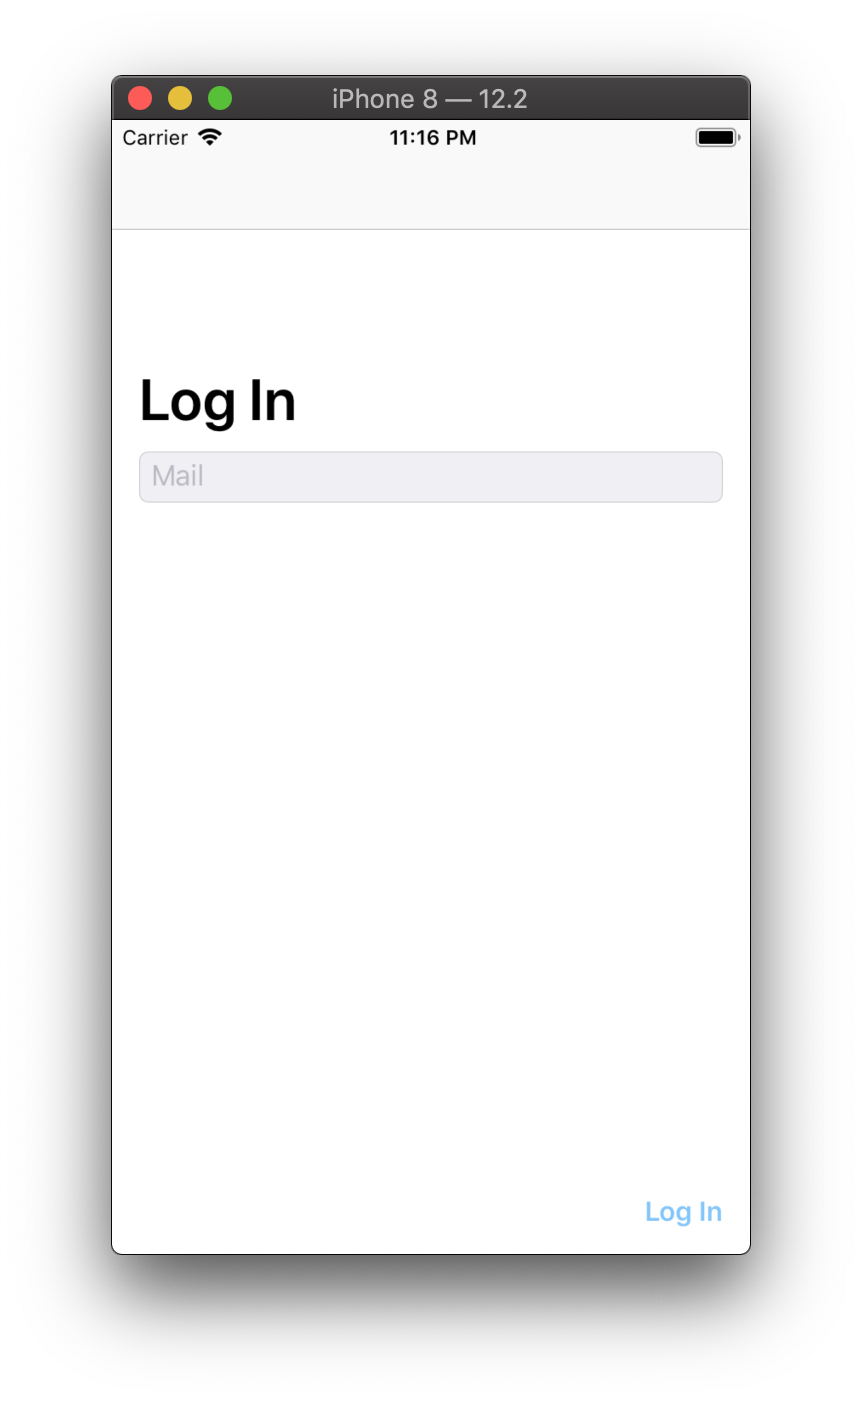
\includegraphics[width=\linewidth]{../includes/pmi/login.png}
		\end{subfigure}
		\begin{subfigure}[b]{0.3\linewidth}
			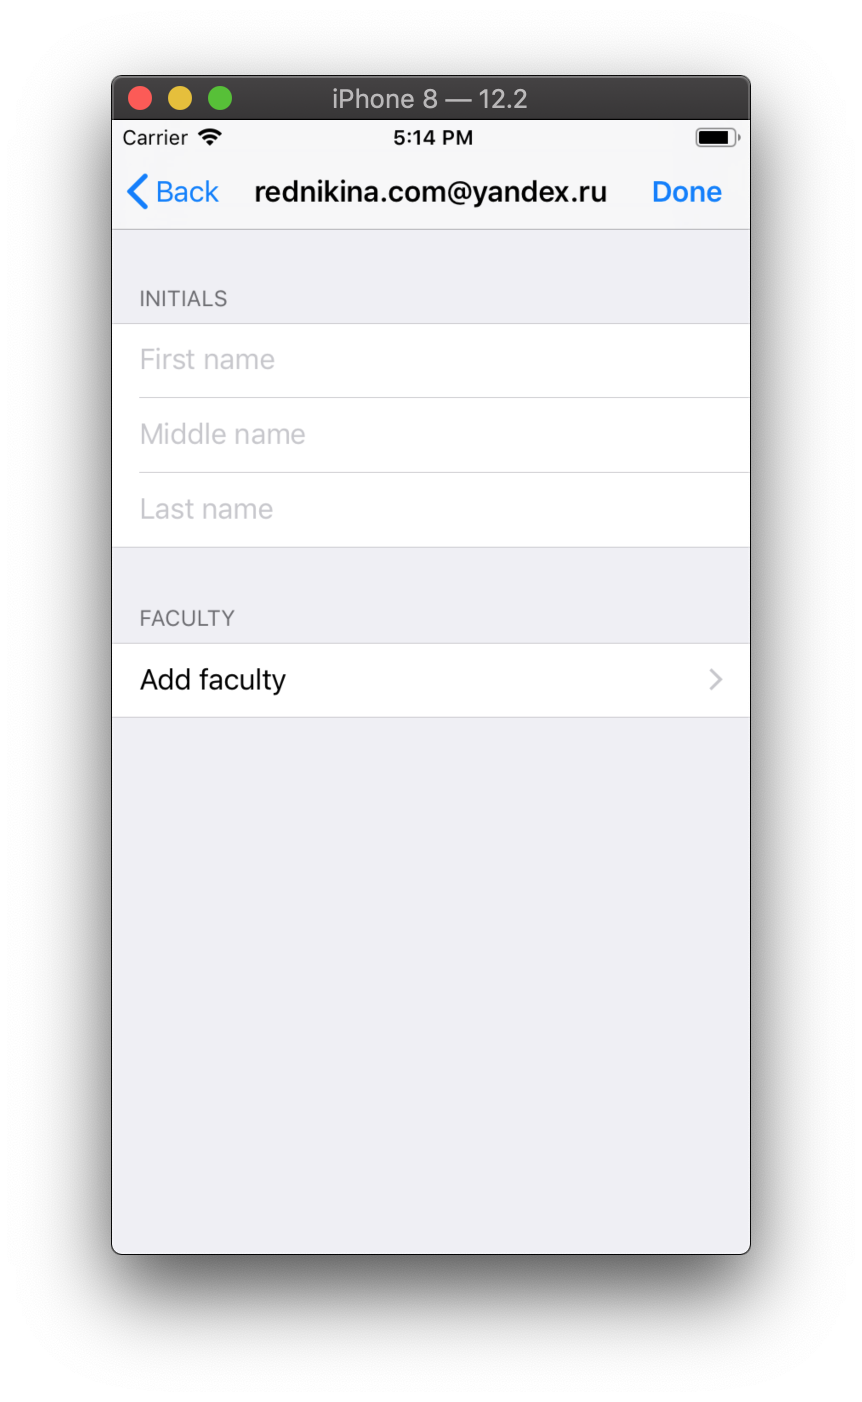
\includegraphics[width=\linewidth]{../includes/pmi/r1.png}
		\end{subfigure}
		\begin{subfigure}[b]{0.3\linewidth}
			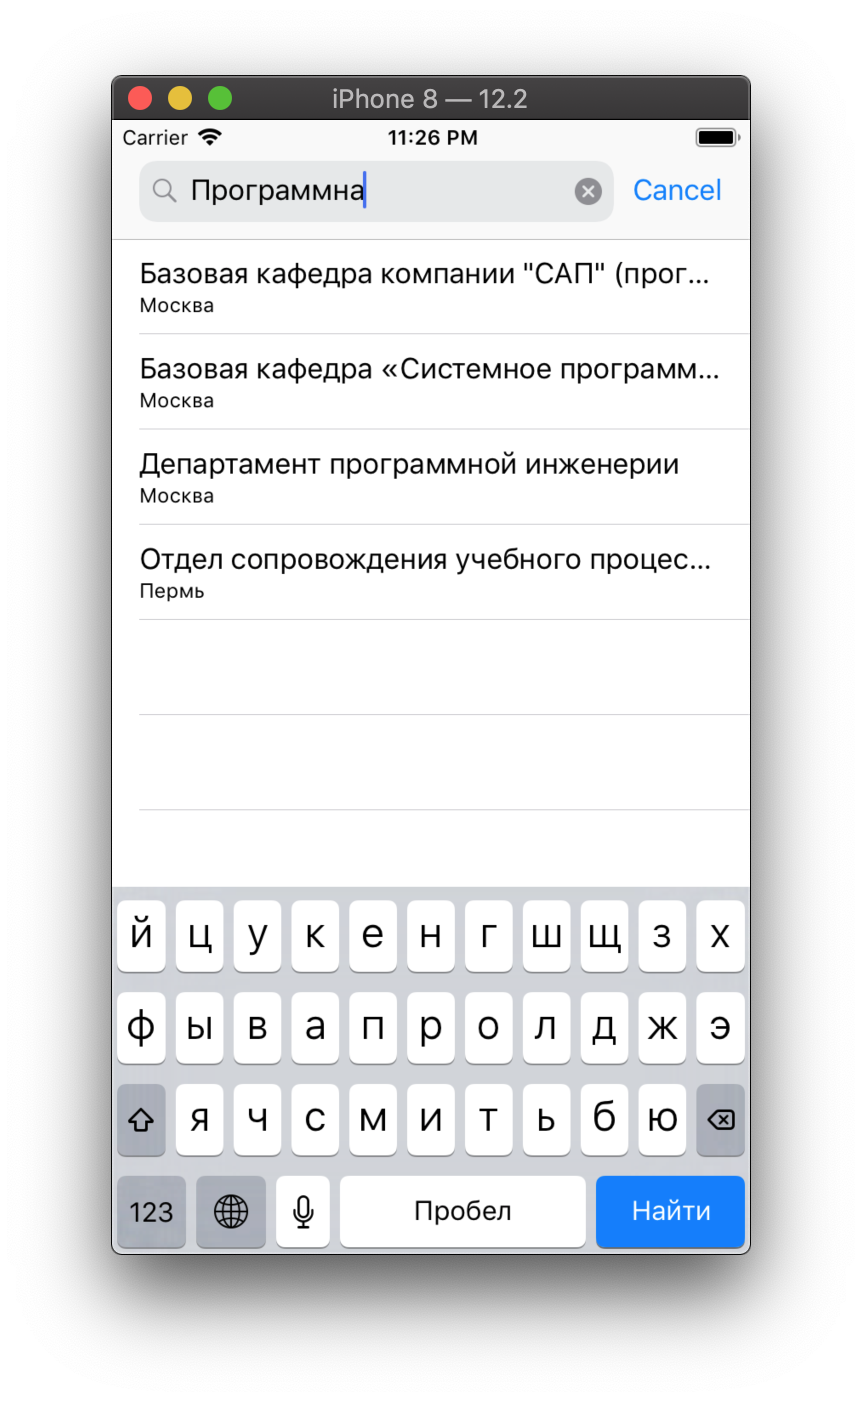
\includegraphics[width=\linewidth]{../includes/pmi/r3.png}
		\end{subfigure}
		\begin{subfigure}[b]{0.3\linewidth}
			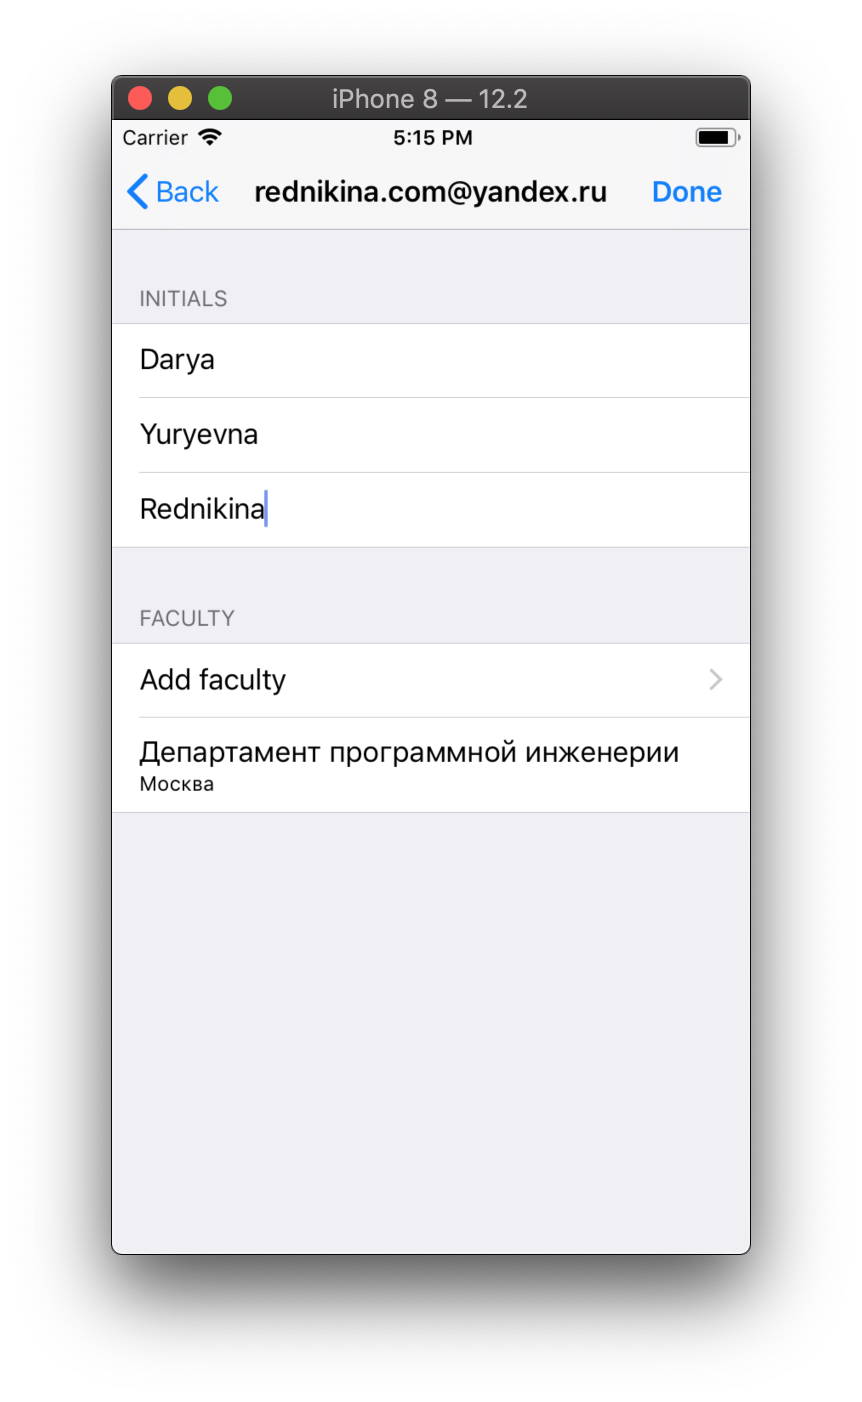
\includegraphics[width=\linewidth]{../includes/pmi/r2.png}
		\end{subfigure}
		\begin{subfigure}[b]{0.3\linewidth}
			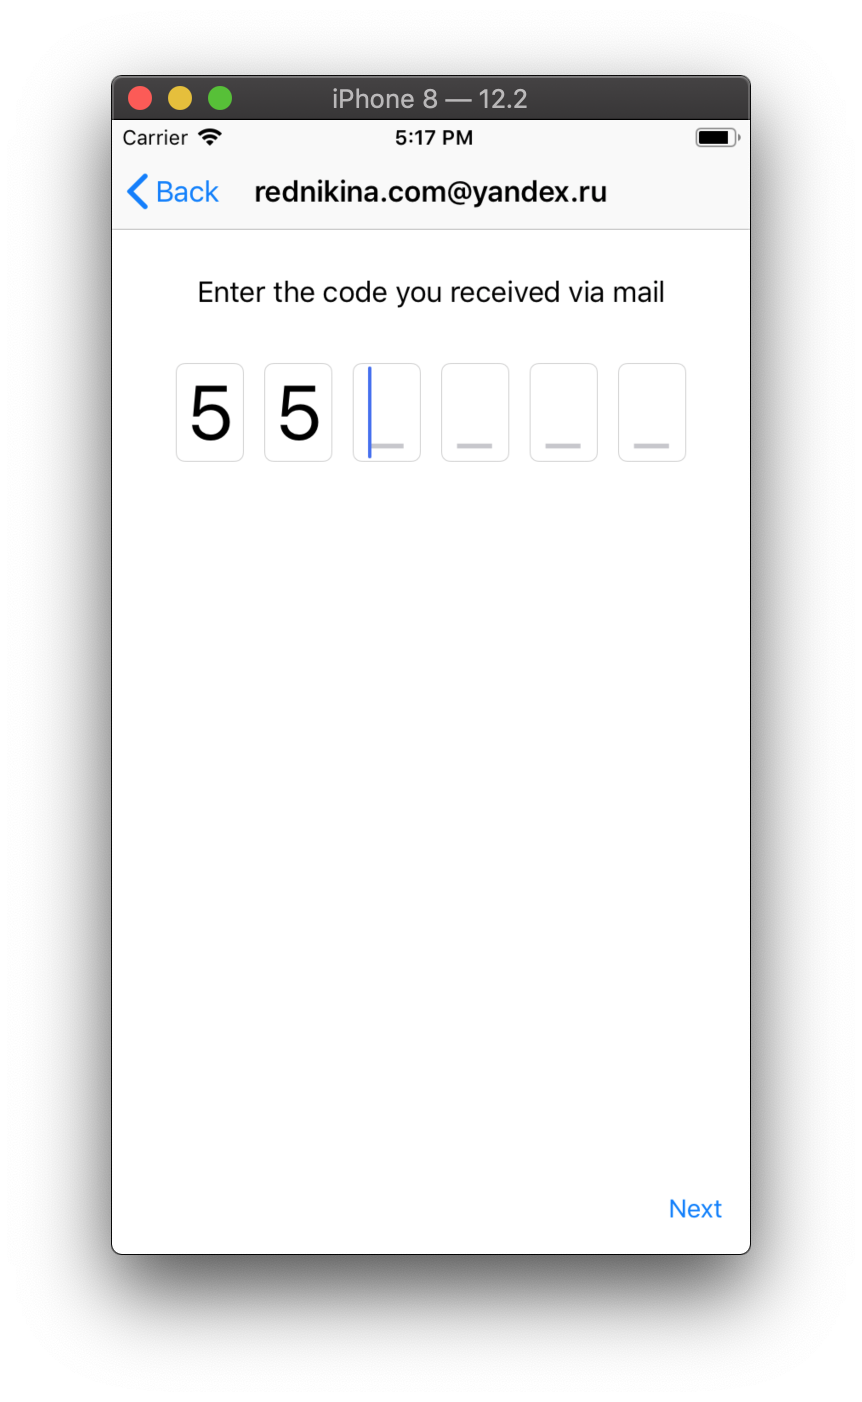
\includegraphics[width=\linewidth]{../includes/pmi/code.png}
		\end{subfigure}
		\caption{\label{pic: register}Регистрация клиента в социальной сети}
	\end{figure}

	Регистрация осуществляется при введении почты с \verb|@hse.ru| в поле для текста на рис. \ref{pic: register}. При успешной валидации почты на сервере \cite{server}, пользователь может ввести свои данные (ФИО, факультет) в поля (см. рис \ref{pic: register}). При успешном заполнении полей (выбран факультет и ФИО введено полностью) пользователь должен ввести код валидации, отправленный на почту, для входа в приложение. Для подтвеждения введенных данных клиент должен нажать кнопку \textit{Next} в правом нижнем углу, при неверно введенном коде пользователю будет отображено сообщение (см. рис \ref{pic: auto}).
	\subsubsection{Авторизация клиента}
	При авторизации пользователь также должен ввести почту \verb|@hse.ru| и код валидации (см. рис. \ref{pic: auto}).
	\begin{figure}[h!]
		\centering
		\begin{subfigure}[b]{0.3\linewidth}
			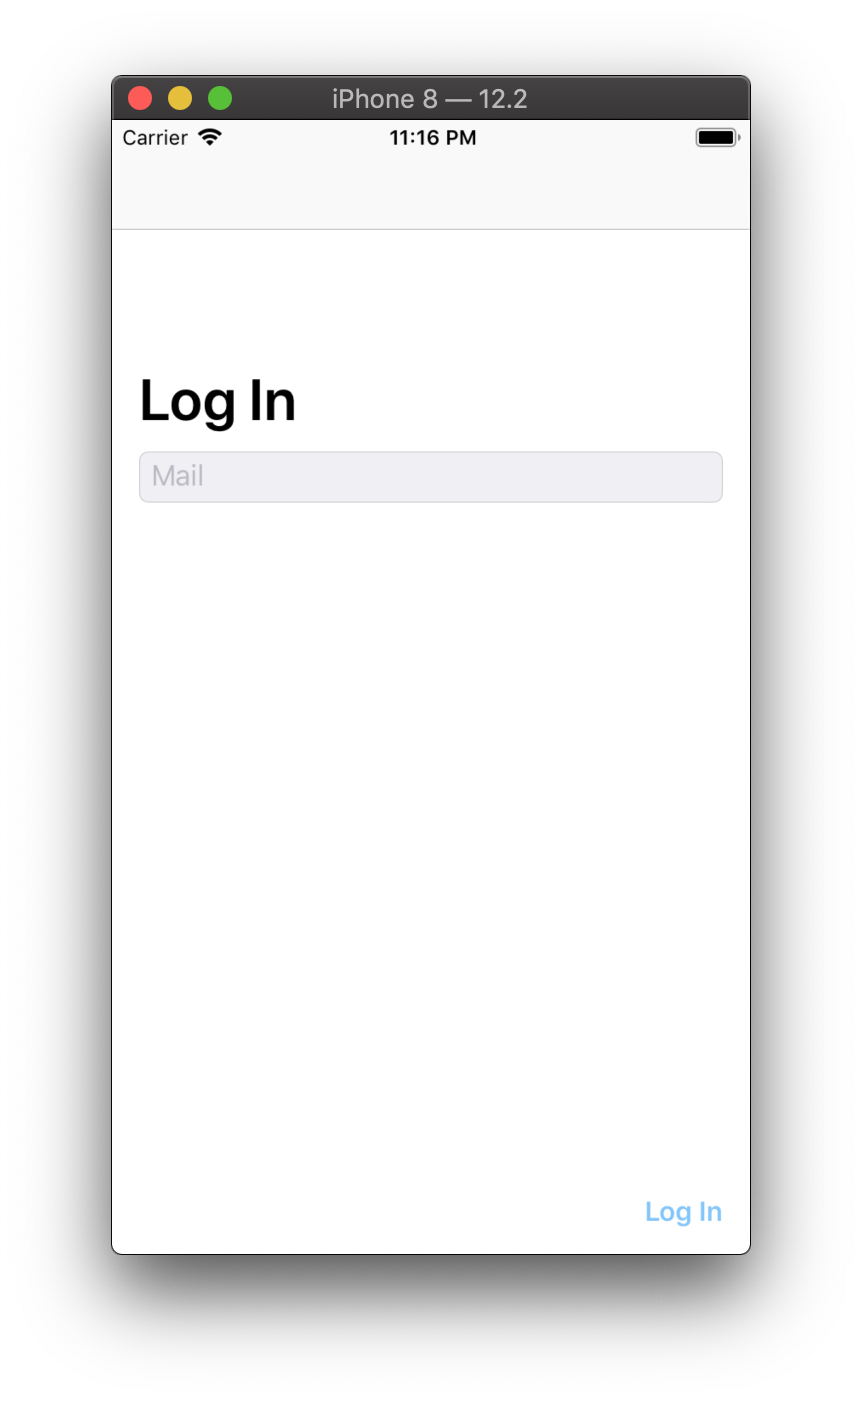
\includegraphics[width=\linewidth]{../includes/pmi/login.png}
		\end{subfigure}
		\begin{subfigure}[b]{0.3\linewidth}
			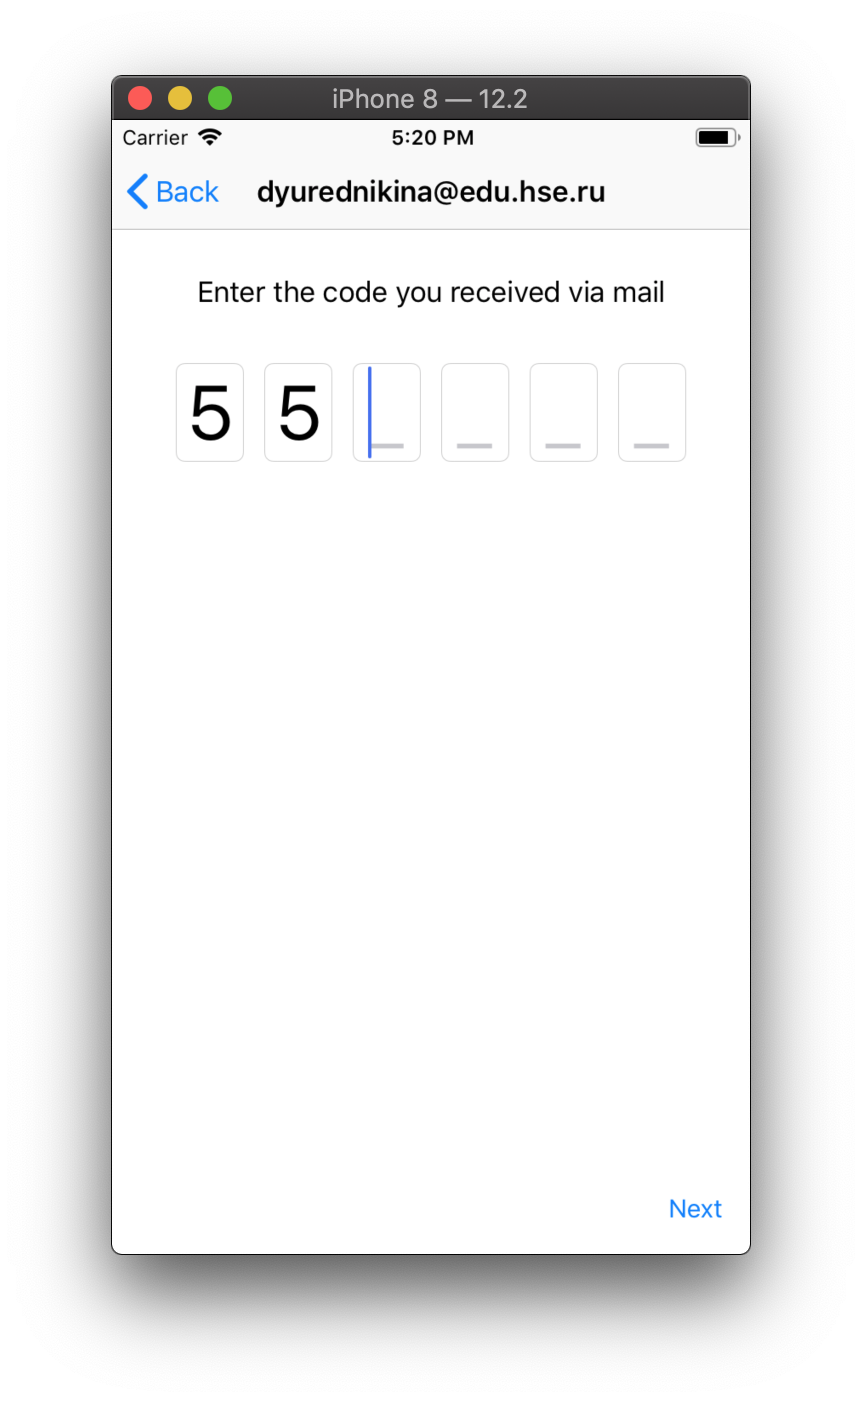
\includegraphics[width=\linewidth]{../includes/pmi/code1.png}
		\end{subfigure}
		\begin{subfigure}[b]{0.3\linewidth}
			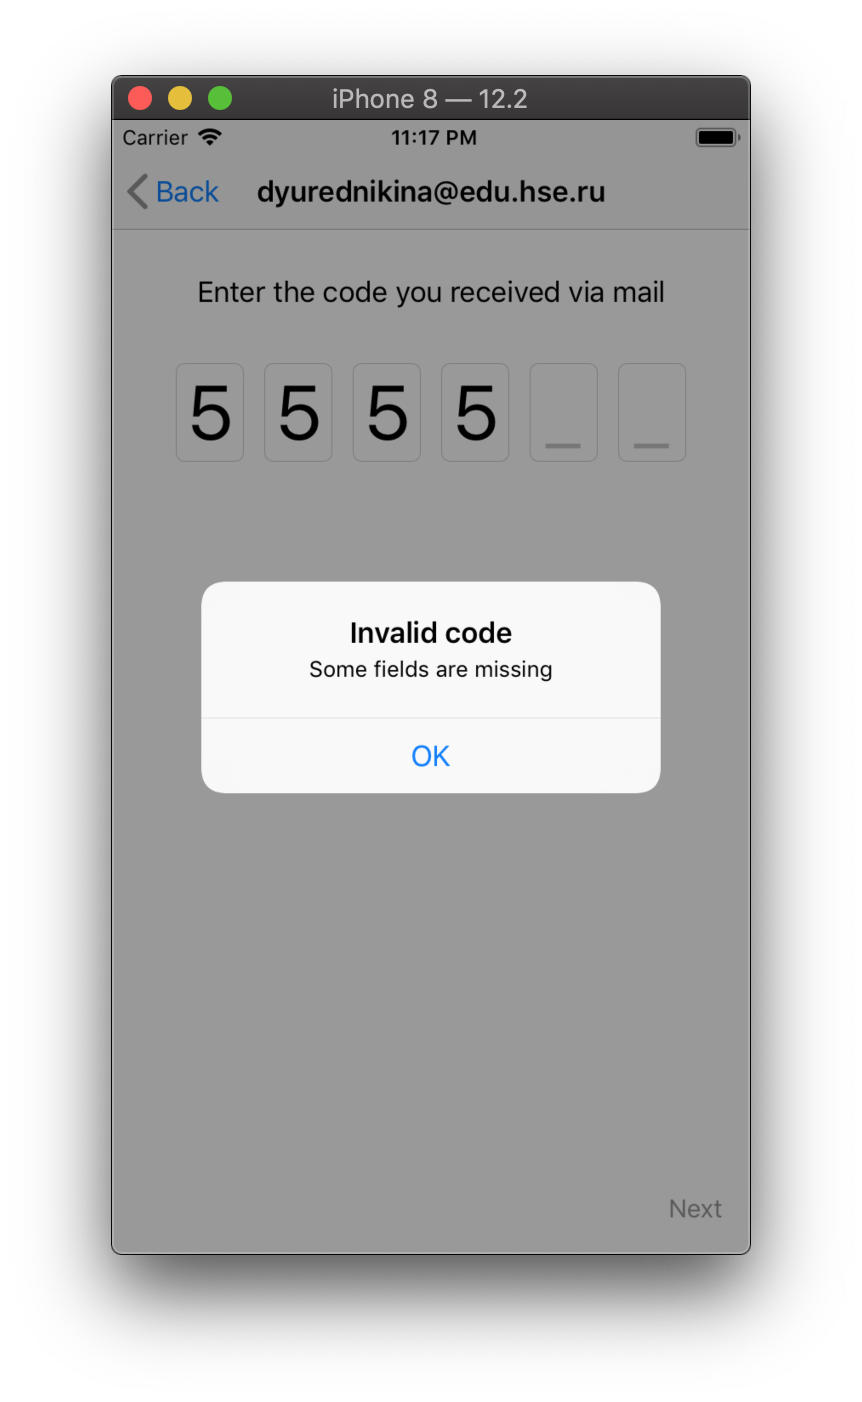
\includegraphics[width=\linewidth]{../includes/pmi/invalidcode.png}
		\end{subfigure}
		\caption{\label{pic: auto} Авторизация клиента в социальной сети}
	\end{figure}
	\clearpage
	\subsubsection{Просмотр профиля пользователя}
	\paragraph{Просмотр своего профиля\\}
	
	При выборе \textit{Profile} на \textit{tabBar}(\ref{C: tabbar}) пользователь оказывается на странице своего профиля: при выборе на \textit{segmented control} секции \textit{Posts} отображаются посты пользователя - по нажатию пост открывается целиком (см. \ref{pic: myprofile}), в секции \textit{Basic info} - информация о контактах, факультете, интересах пользователя. При выборе \textit{More} в правом верхнем углу появляется \textit{Action sheet}(\ref{C: actionSheet}) для предоставления выбора действий со своей страницы: выйти из аккаунта, выйти из аккаунта со всех устройств или редактировать информацию о себе. При редактировании информации о себе появляется окошко для редактирования (см. \ref{pic: myprofile}). Сохранение отредактированной информации происходит при нажатии на кнопку \textit{Done}.
	
	\begin{figure}[h!]
		\centering
		\begin{subfigure}[b]{0.3\linewidth}
			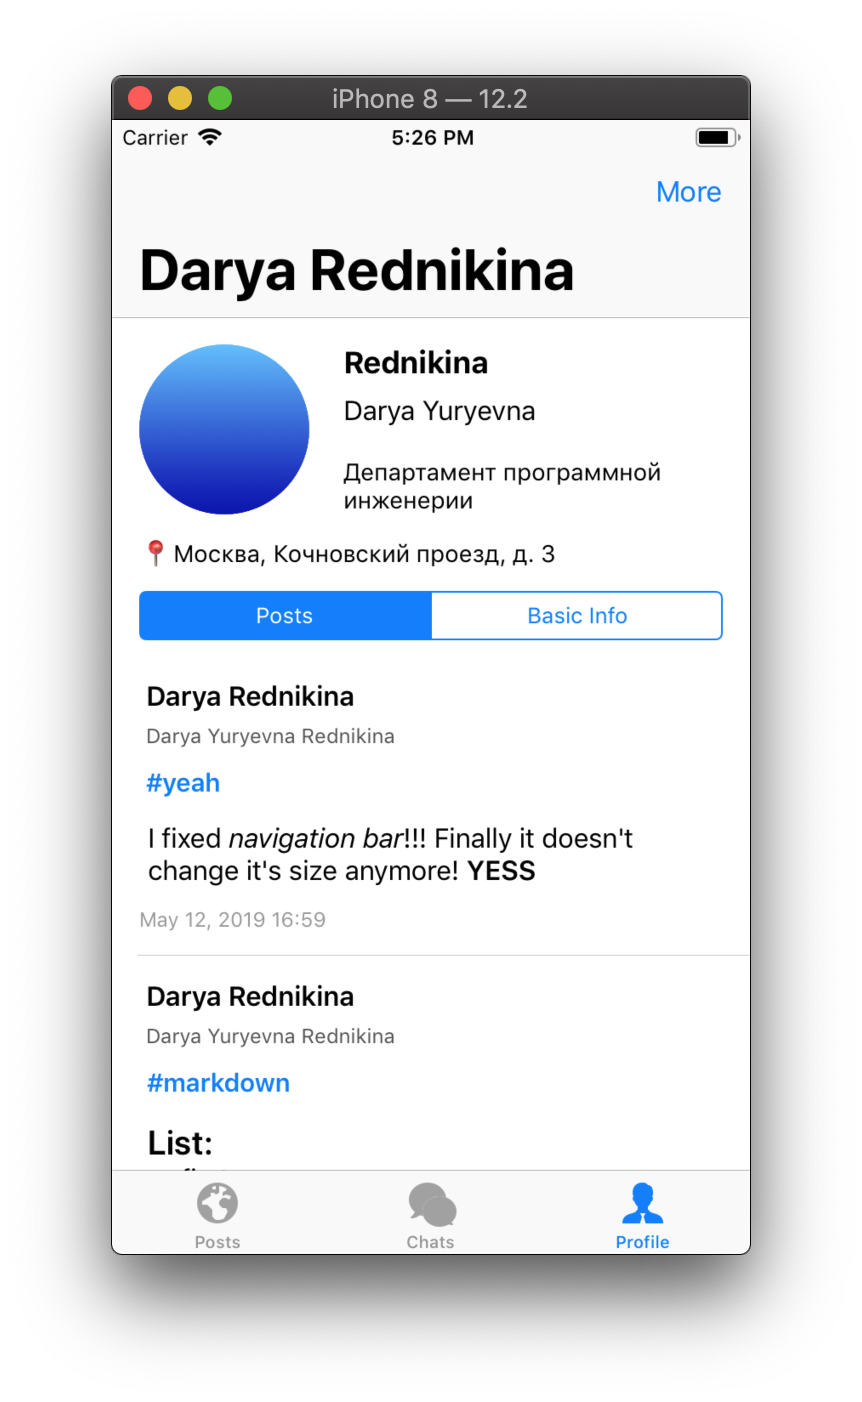
\includegraphics[width=\linewidth]{../includes/pmi/profile.png}
		\end{subfigure}
		\begin{subfigure}[b]{0.3\linewidth}
			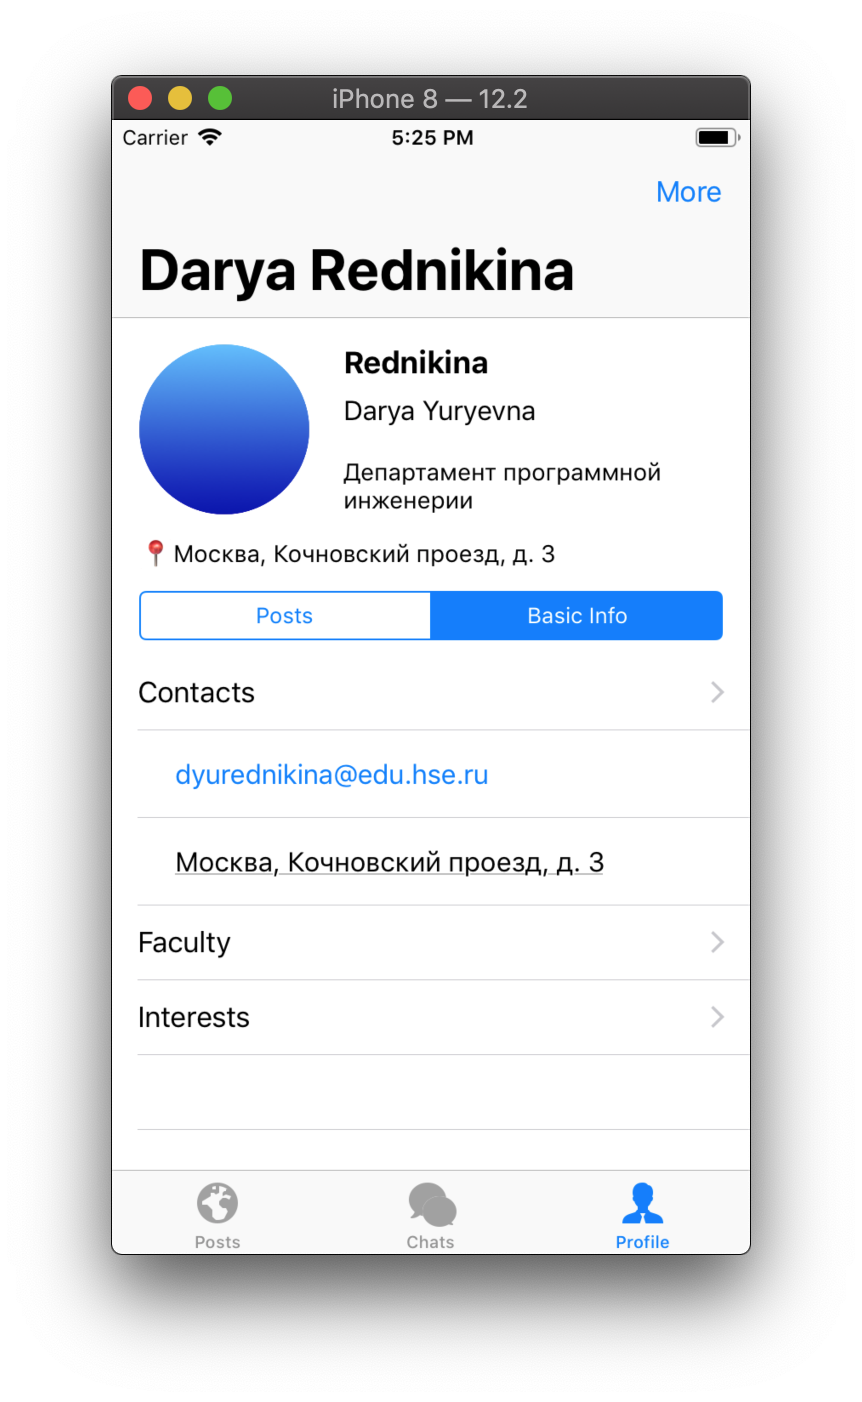
\includegraphics[width=\linewidth]{../includes/pmi/basic_info.png}
		\end{subfigure}
		\begin{subfigure}[b]{0.3\linewidth}
			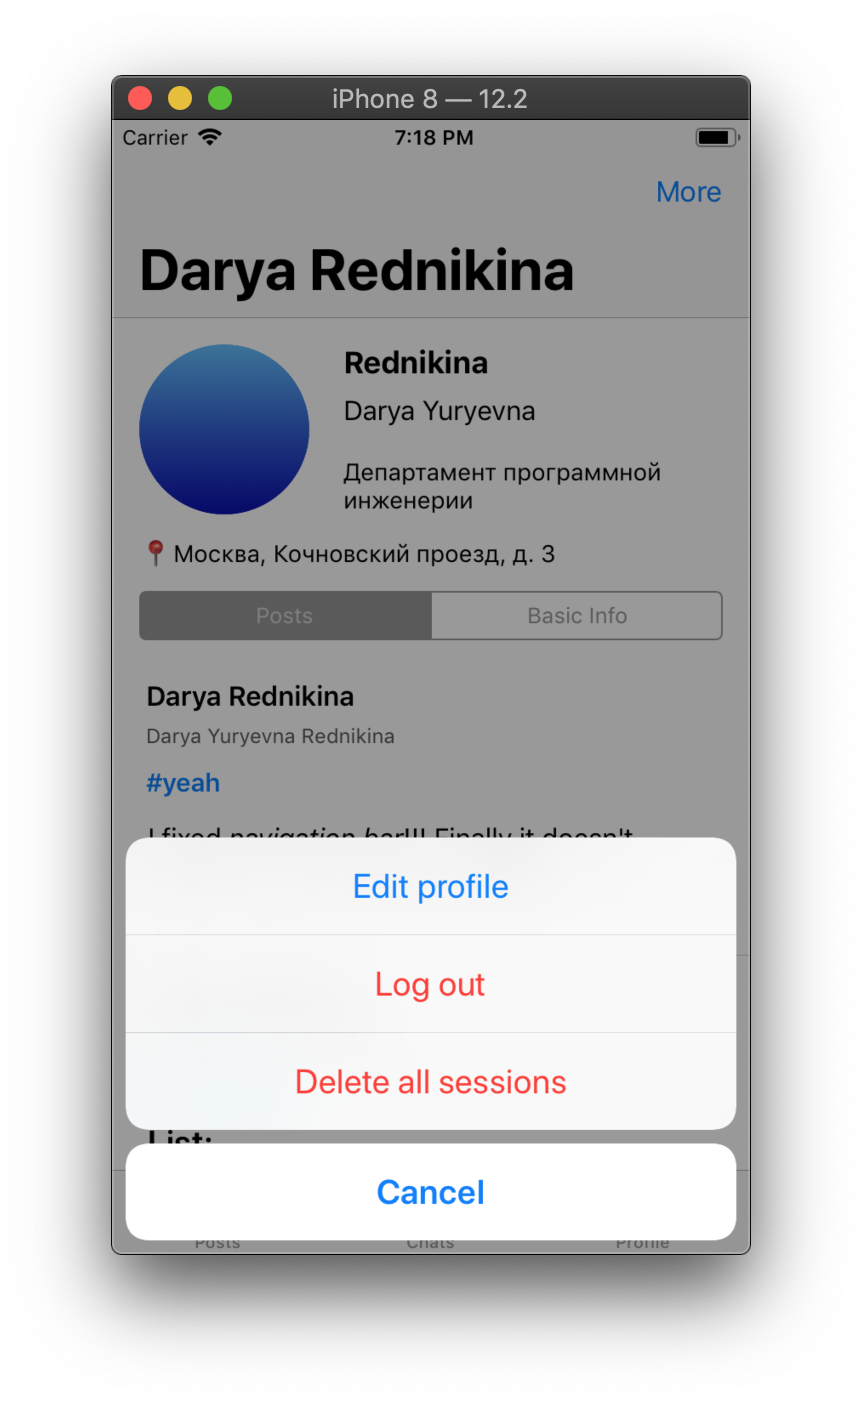
\includegraphics[width=\linewidth]{../includes/pmi/profile_functions.png}
		\end{subfigure}
		\begin{subfigure}[b]{0.3\linewidth}
			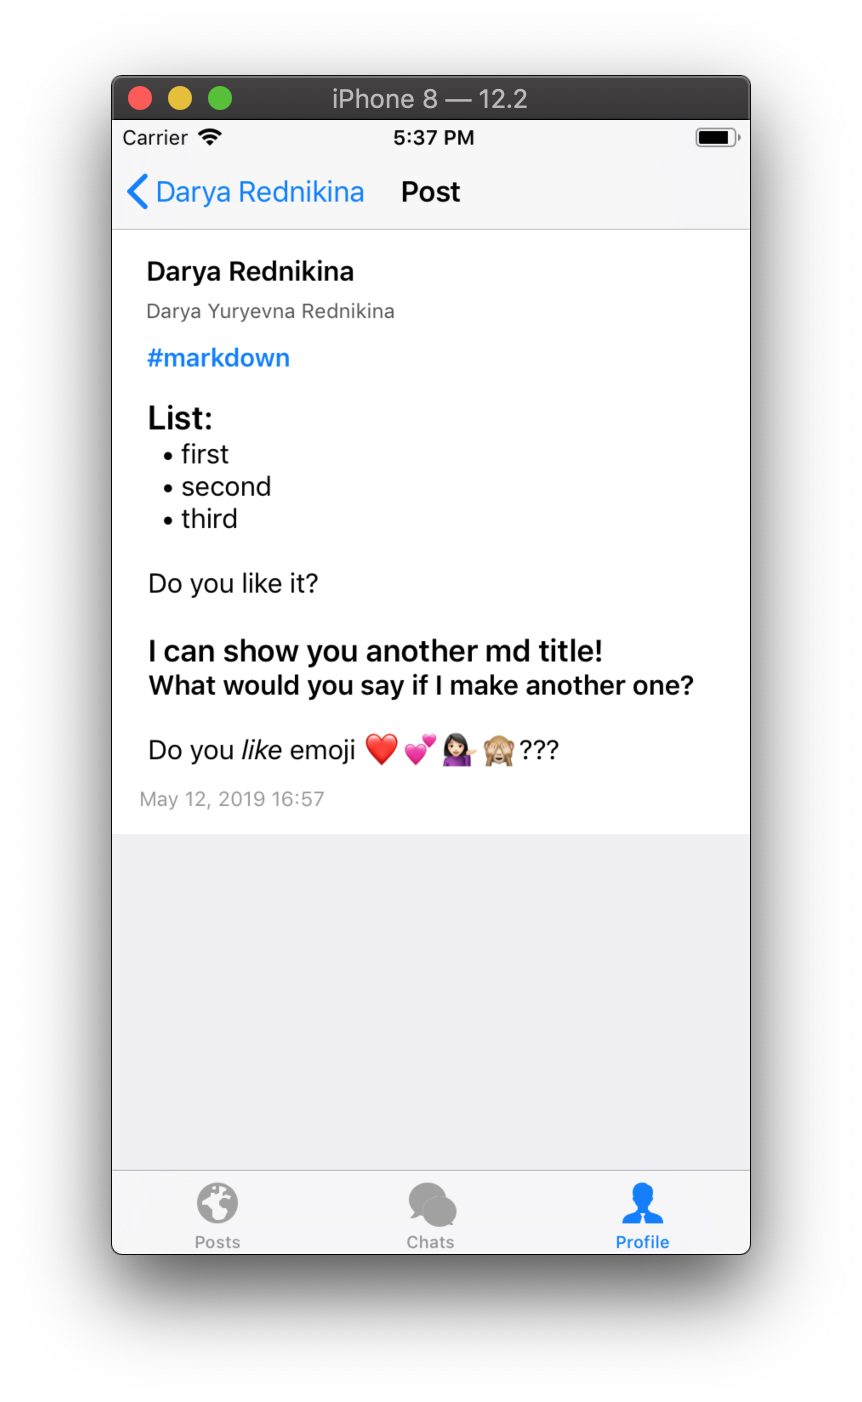
\includegraphics[width=\linewidth]{../includes/pmi/profile_fullpost.png}
		\end{subfigure}
		\begin{subfigure}[b]{0.3\linewidth}
			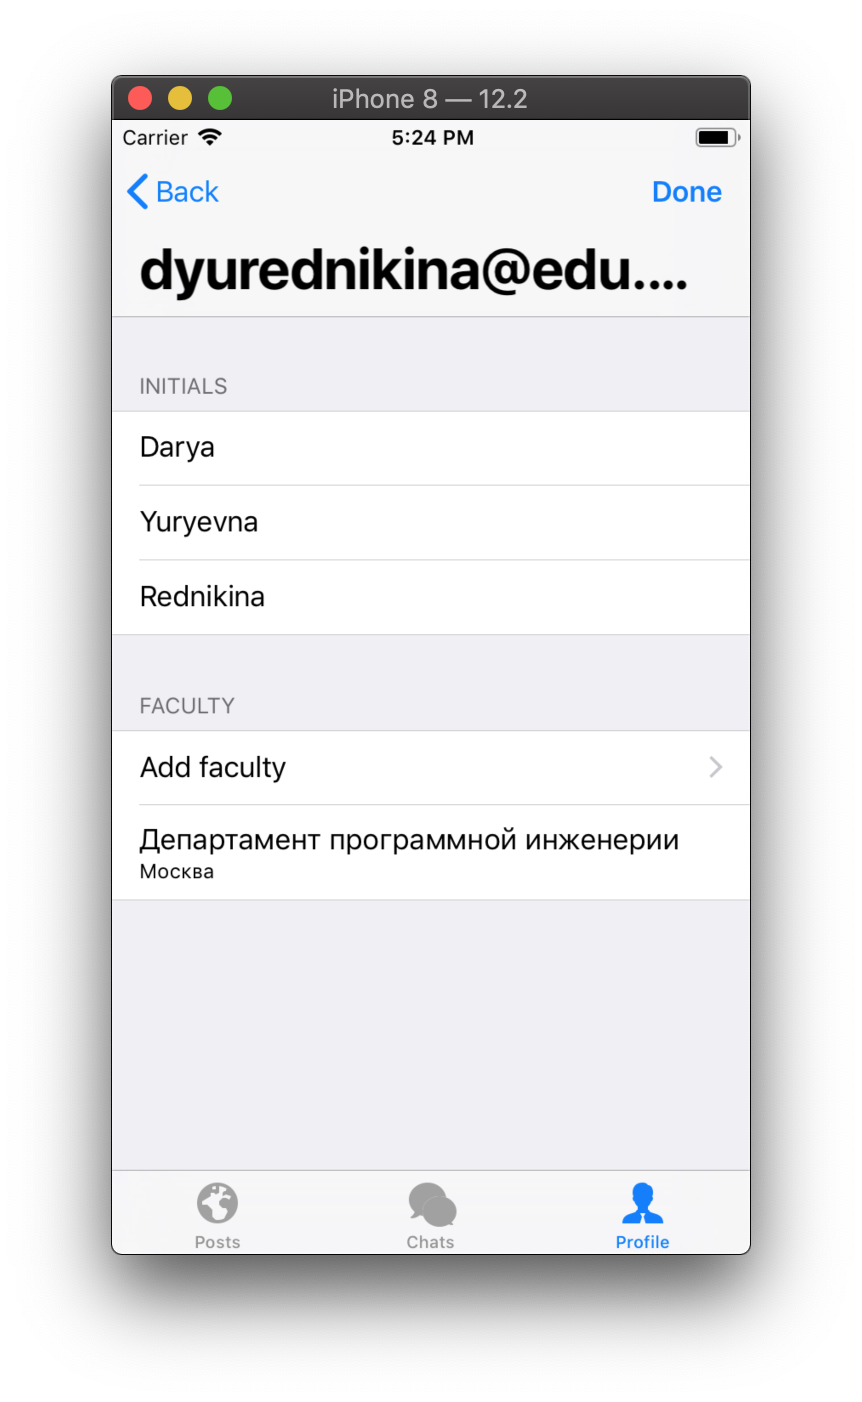
\includegraphics[width=\linewidth]{../includes/pmi/edit_profile.png}
		\end{subfigure}

		\caption{\label{pic: myprofile} Просмотр своего профиля}
	\end{figure}
	\clearpage
	\paragraph{Просмотр профилей других пользователей\\}
	При просмотре общей ленты, сообщений в диалогах, канала можно перейти на профиль автора поста/сообщения (при нажатии на имя автора). Если автором не является авторизованный пользователь, то в профиле есть возможность написать человеку сообщение (см. \ref{pic: otherprofile}) при нажатии кнопки \textit{New message}. Также доступны вышеперечисленные (см. \ref{pic: myprofile}) возможности просмотра постов, информации о человеке на его странице. Но \textit{Action sheet}(\ref{C: actionSheet}) содержит опцию добавления профиля в один из существующих каналов (см. \ref{pic: otherprofile}), которая доступна при нажатии на опцию \textit{Add to a channel}.
	
	\begin{figure}[h!]
	\centering
	\begin{subfigure}[b]{0.3\linewidth}
		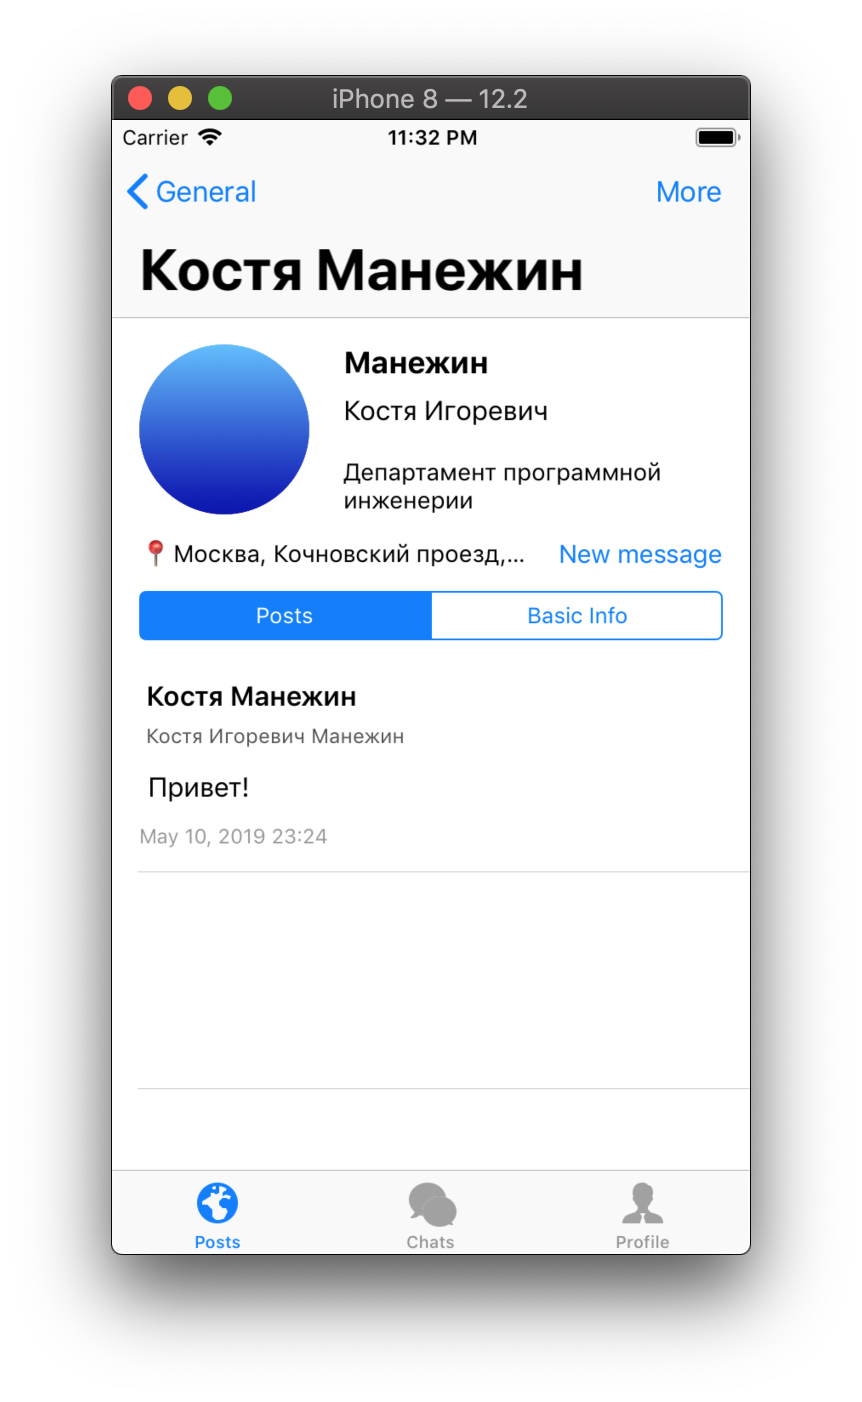
\includegraphics[width=\linewidth]{../includes/pmi/otherprofile.png}
	\end{subfigure}
	\begin{subfigure}[b]{0.3\linewidth}
		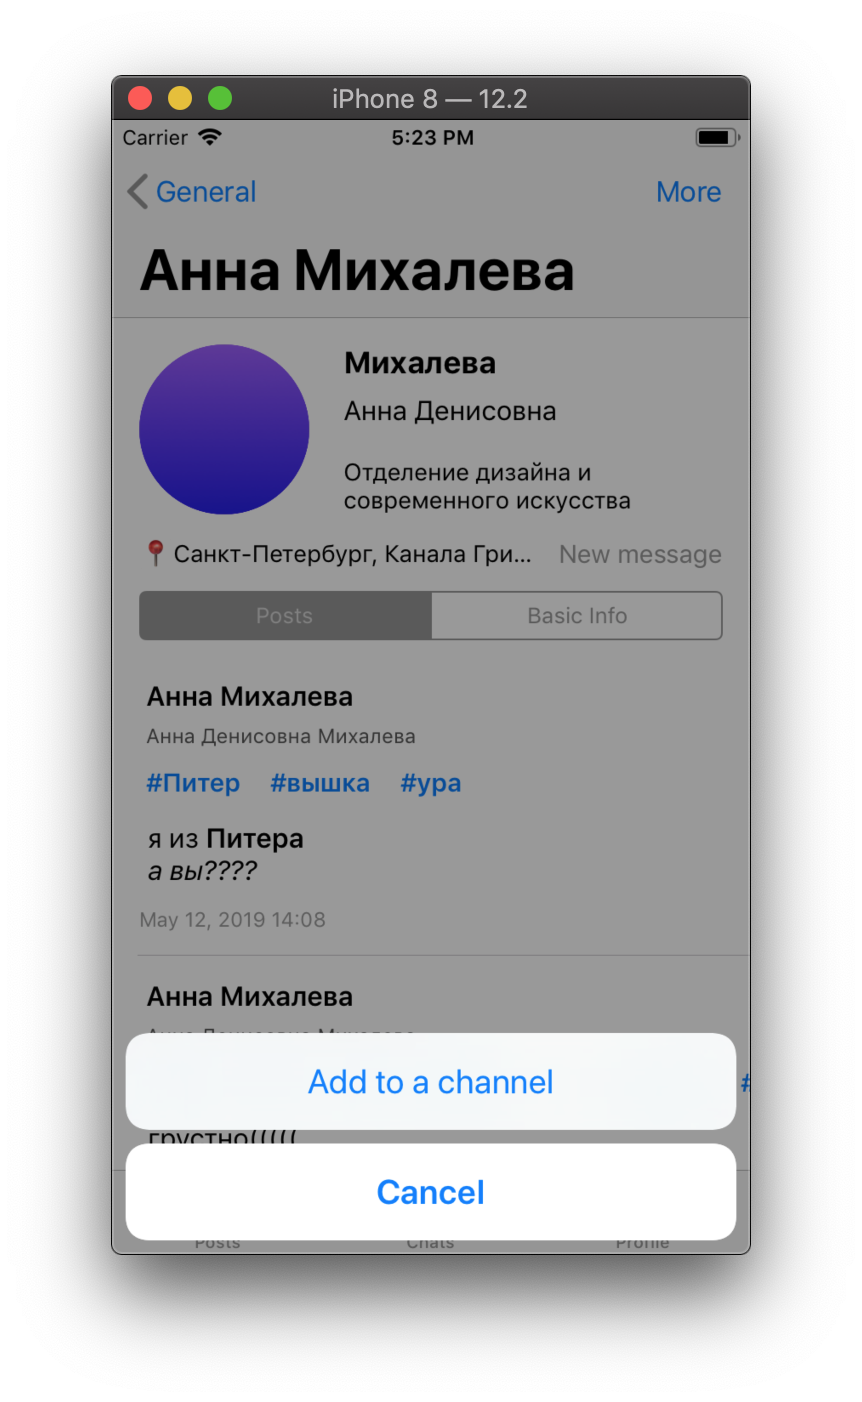
\includegraphics[width=\linewidth]{../includes/pmi/otherprofile_functions.png}
	\end{subfigure}
	\begin{subfigure}[b]{0.3\linewidth}
		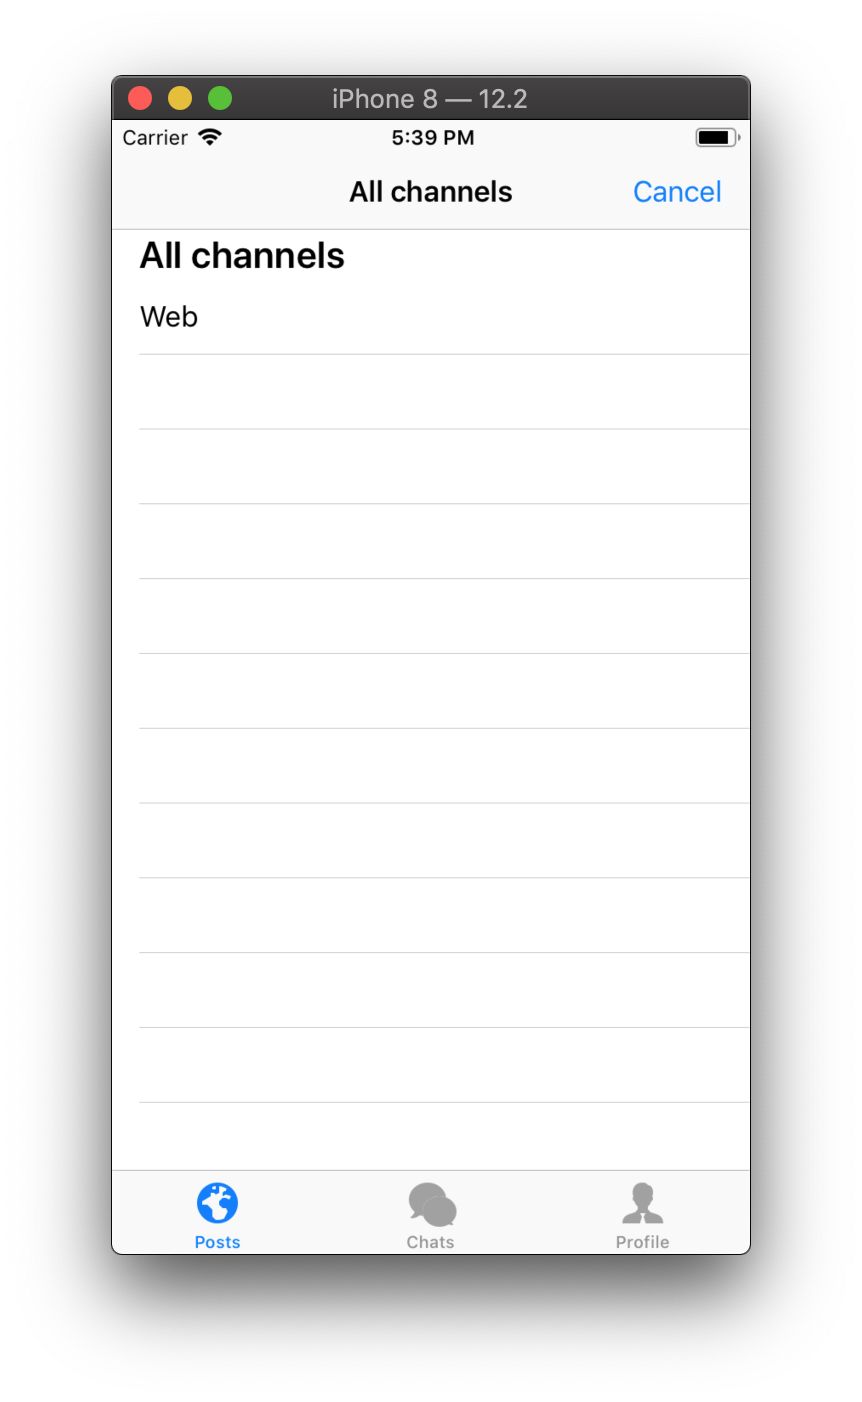
\includegraphics[width=\linewidth]{../includes/pmi/addtoachannel.png}
	\end{subfigure}
	\caption{\label{pic: otherprofile} Просмотр профилей других пользователей}
	\end{figure}
	\clearpage
	\subsubsection{Публикация постов}
	При нажатии в правом верхнем углу окна с лентой кнопки (cм. рис \ref{pic: hash}) открывается окно для написания поста. При нажатии кнопки \textit{Edit hashtags} в окне предоставляется окно с возможностью выбрать хэштеги из предложенных или написать свои (см. рис. \ref{pic: hash}). Публикация поста происходит при нажатии кнопки \textit{Post} в правом верхнем углу.
	\begin{figure}[h!]
		\centering
		\begin{subfigure}[b]{0.3\linewidth}
			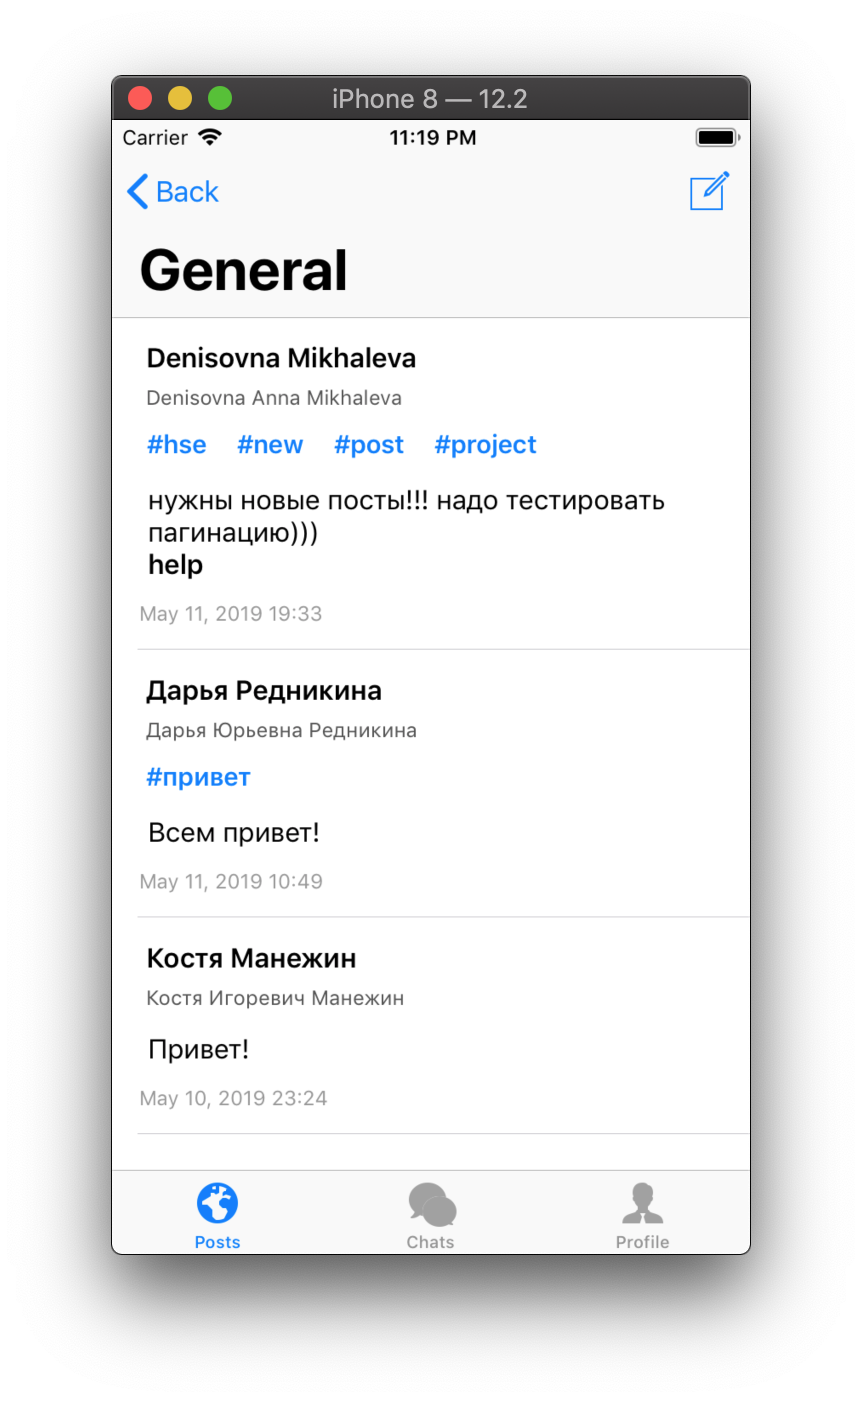
\includegraphics[width=\linewidth]{../includes/pmi/general.png}
		\end{subfigure}
		\begin{subfigure}[b]{0.3\linewidth}
			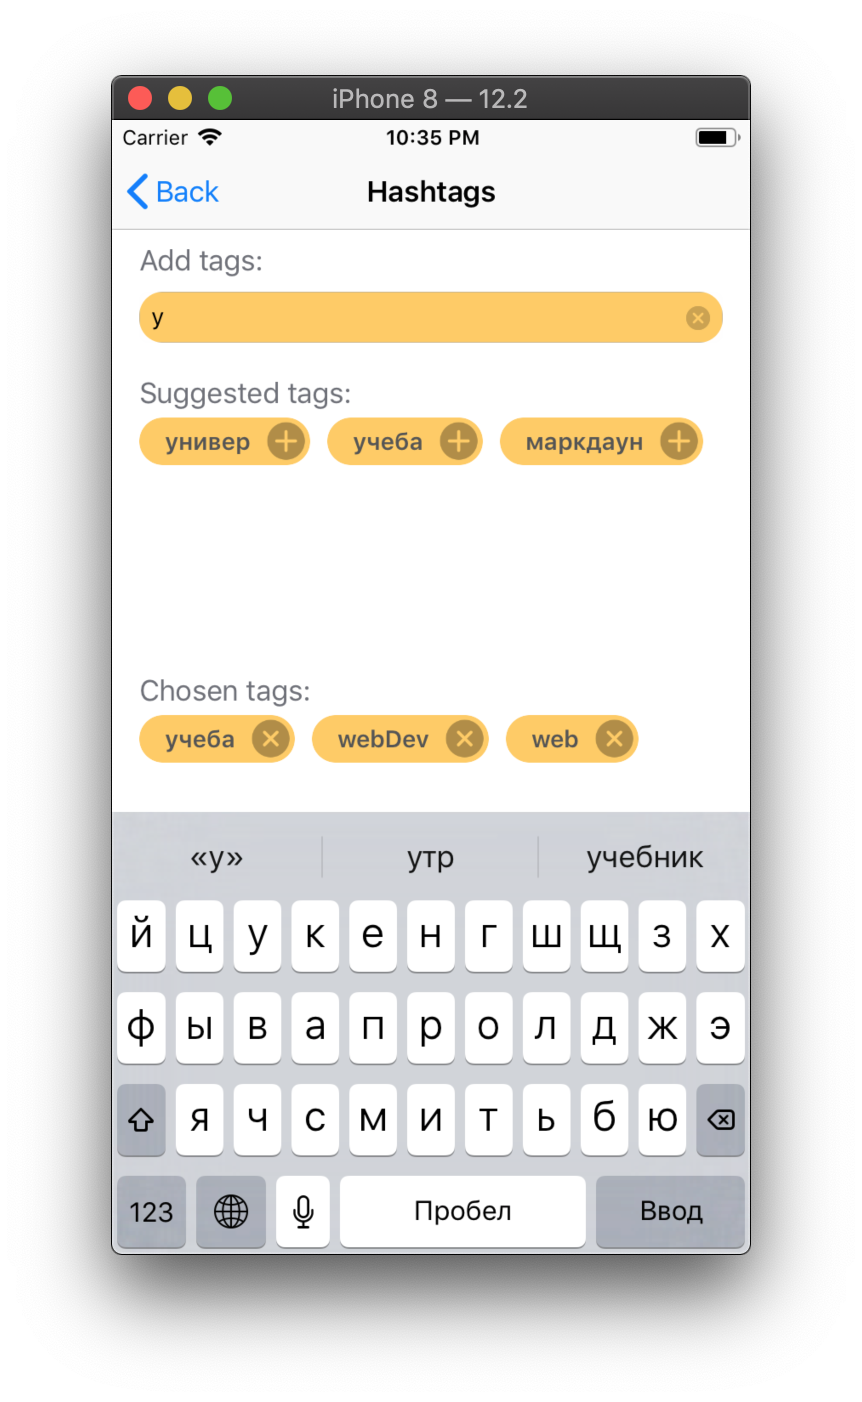
\includegraphics[width=\linewidth]{../includes/pmi/choose_hashtag.png}
		\end{subfigure}
		\caption{\label{pic: hash}Написание поста}
	\end{figure}
	\clearpage
	\subsubsection{Просмотр ленты}
	При просмотре ленты пользователь имеет возможность в строке поиска (см. рис. \ref{pic: newss}) выбрать хэштег для отображения ленты, состоящей из постов, содержащих этот хэштег. Также при просмотре ленты при нажатии на ячейку с постом можно перейти на отображение полного содежания поста (см. рис. \ref{pic: newss}).  При нажатии на хэштег в общей ленте происходит отображение ленты постов, содержащих этот хэштег (см. рис. \ref{pic: newss}).
	\begin{figure}[h!]
		\centering
		\begin{subfigure}[b]{0.3\linewidth}
			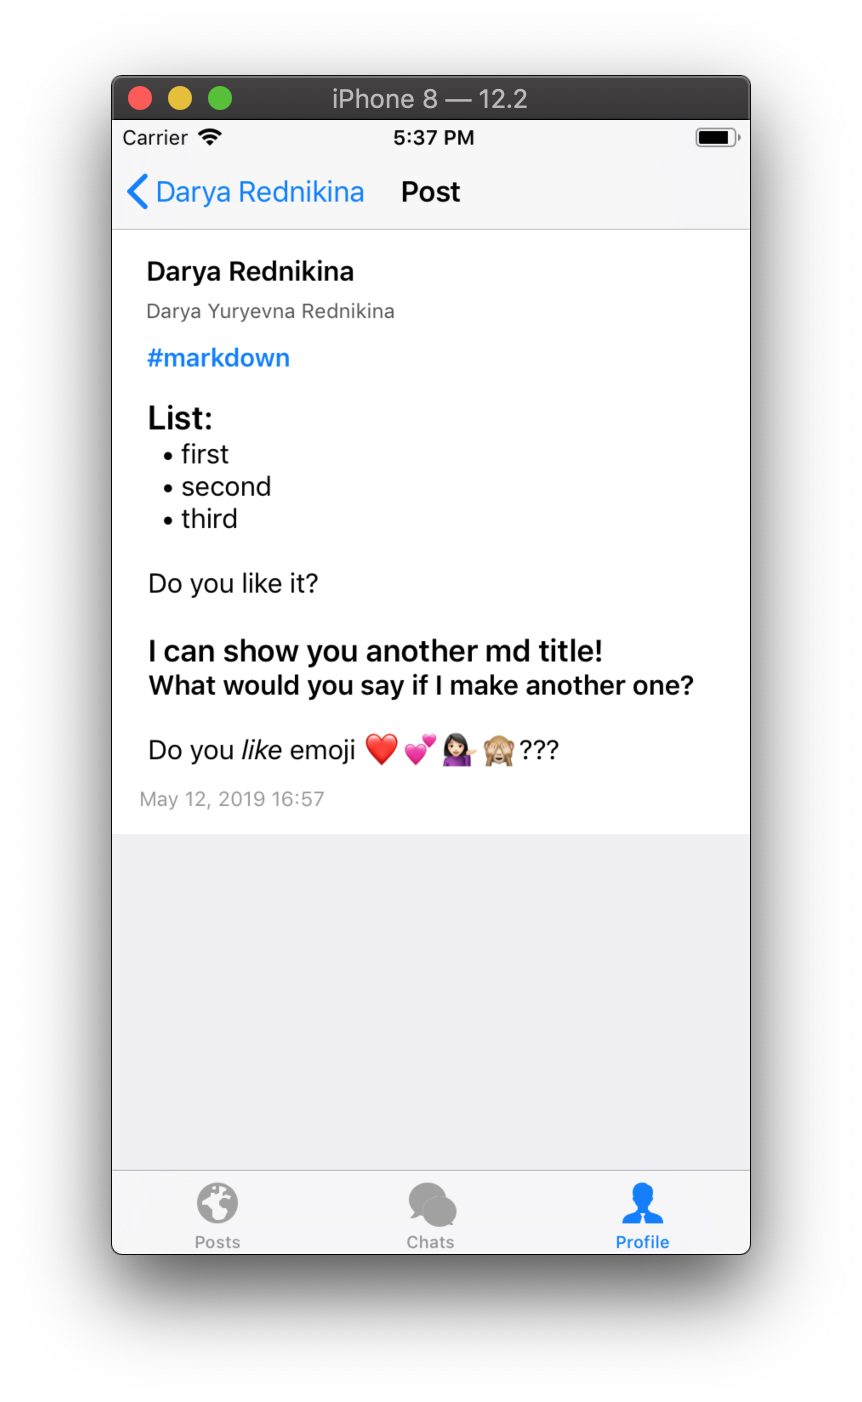
\includegraphics[width=\linewidth]{../includes/pmi/profile_fullpost.png}
		\end{subfigure}
		\begin{subfigure}[b]{0.3\linewidth}
			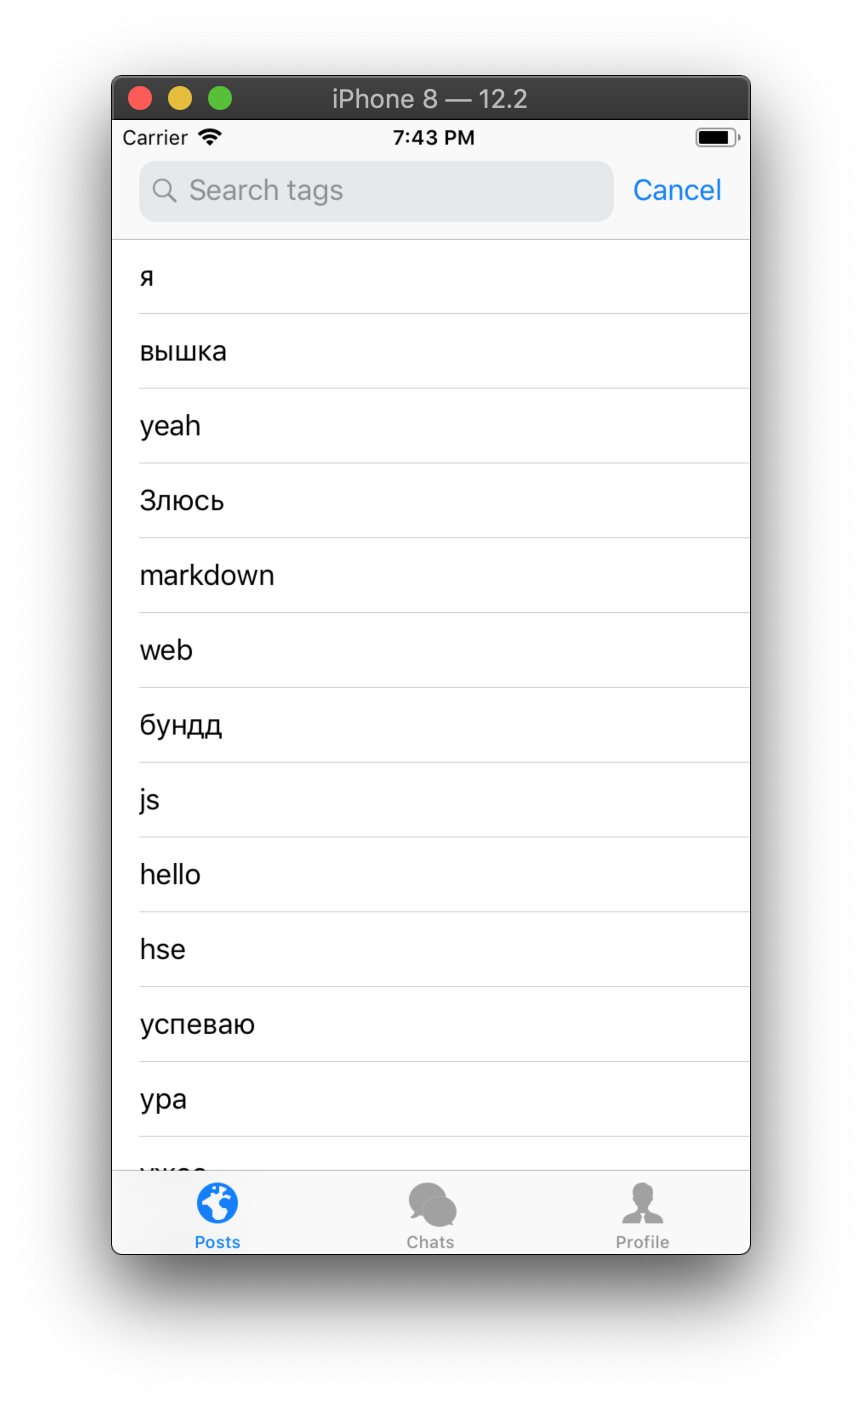
\includegraphics[width=\linewidth]{../includes/pmi/search.png}
		\end{subfigure}
		\begin{subfigure}[b]{0.3\linewidth}
			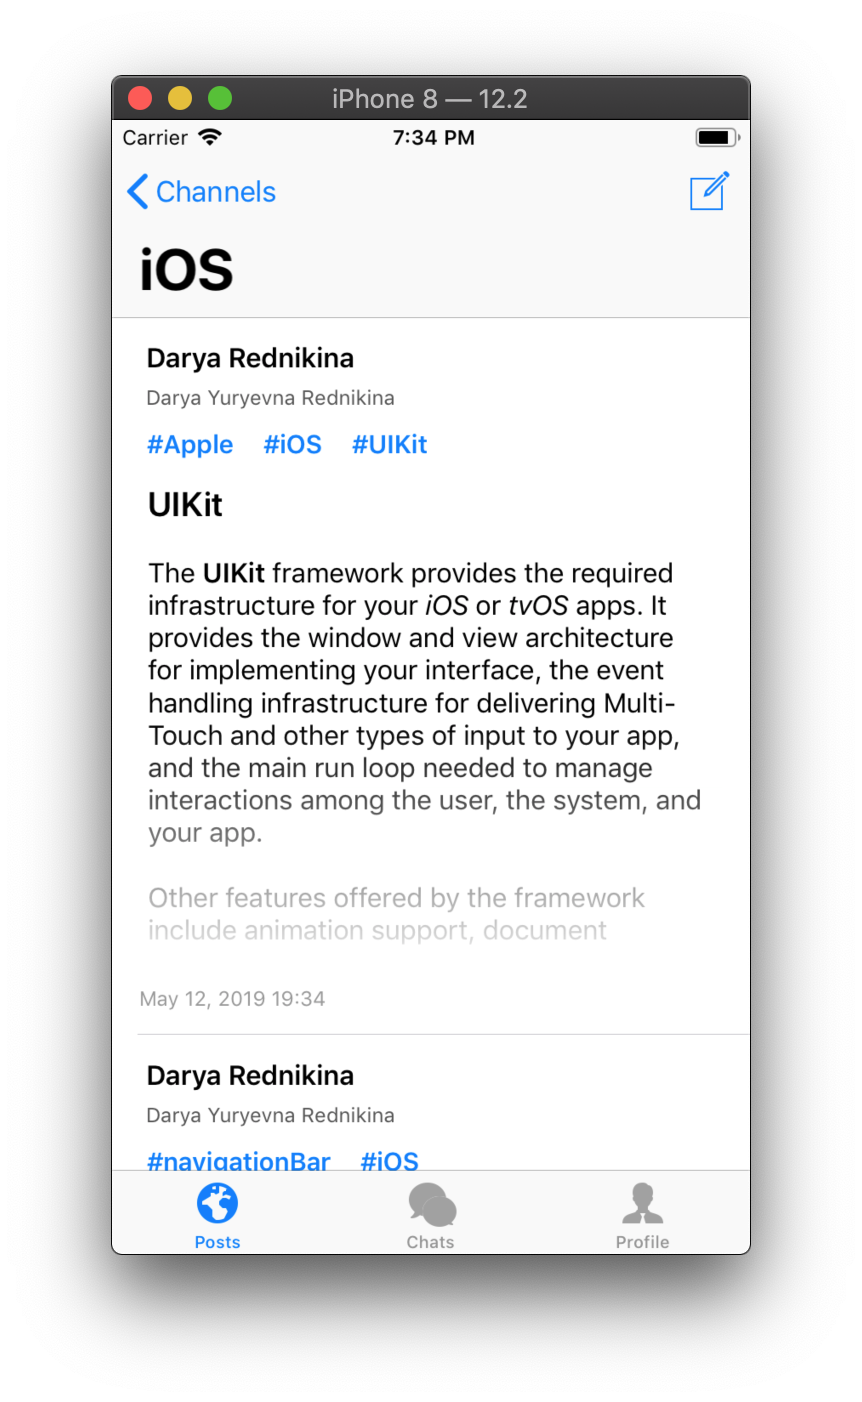
\includegraphics[width=\linewidth]{../includes/pmi/ios_channel.png}
		\end{subfigure}
		\caption{\label{pic: newss}Просмотр ленты}
	\end{figure}
	\clearpage
	\subsubsection{Каналы: создание, удаление и просмотр}
	\paragraph{Создание канала\\}
	При нажатии на кнопку <<+>> в правом верхнем углу открывается окно создания нового канала. В данном окне можно отредактировать название, добавить в список людей и хэштеги. 
	\begin{figure}[h!]
		\centering
		\begin{subfigure}[b]{0.3\linewidth}
			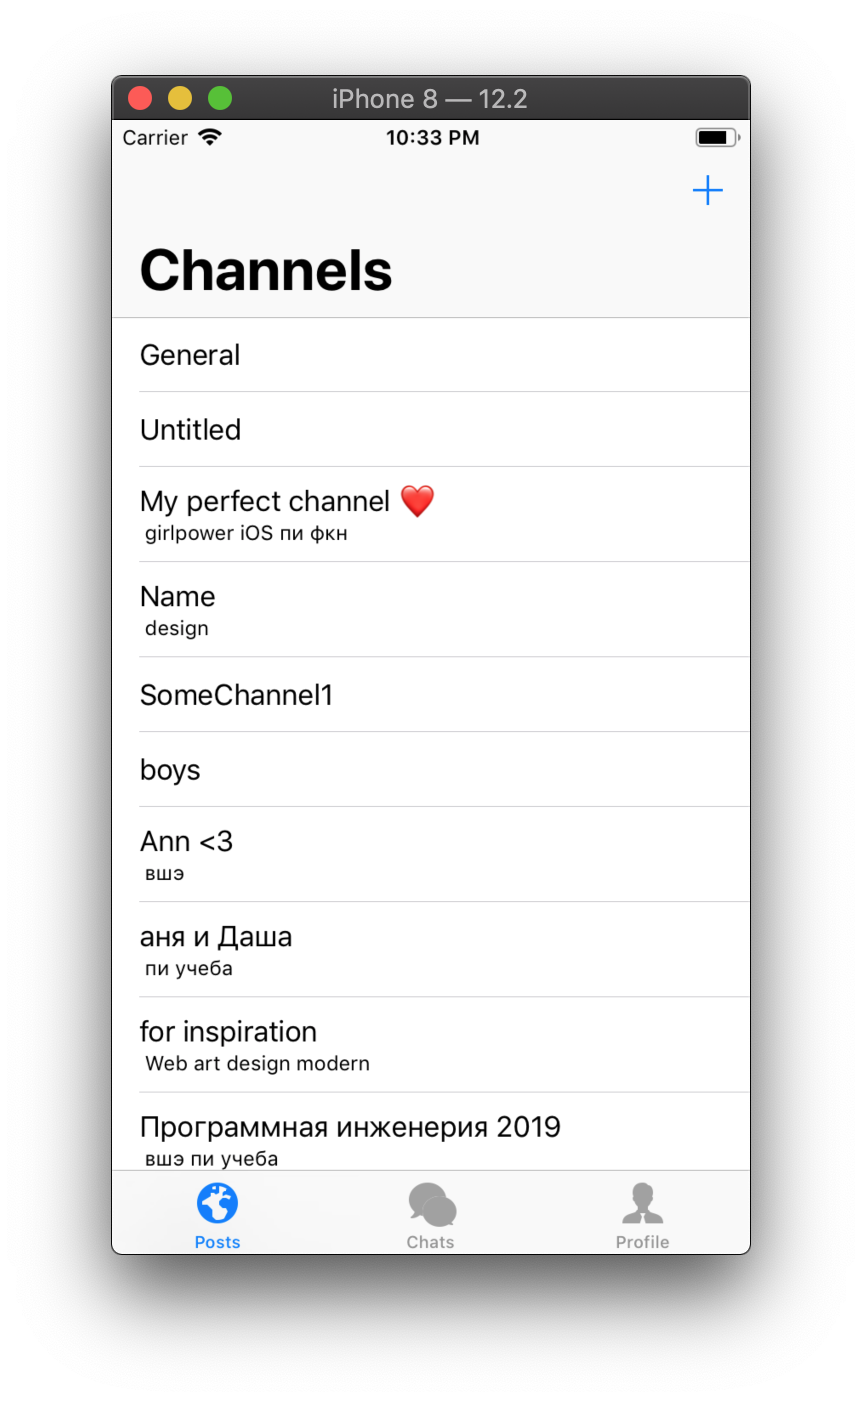
\includegraphics[width=\linewidth]{../includes/pmi/channel_list.png}
		\end{subfigure}
		\begin{subfigure}[b]{0.3\linewidth}
			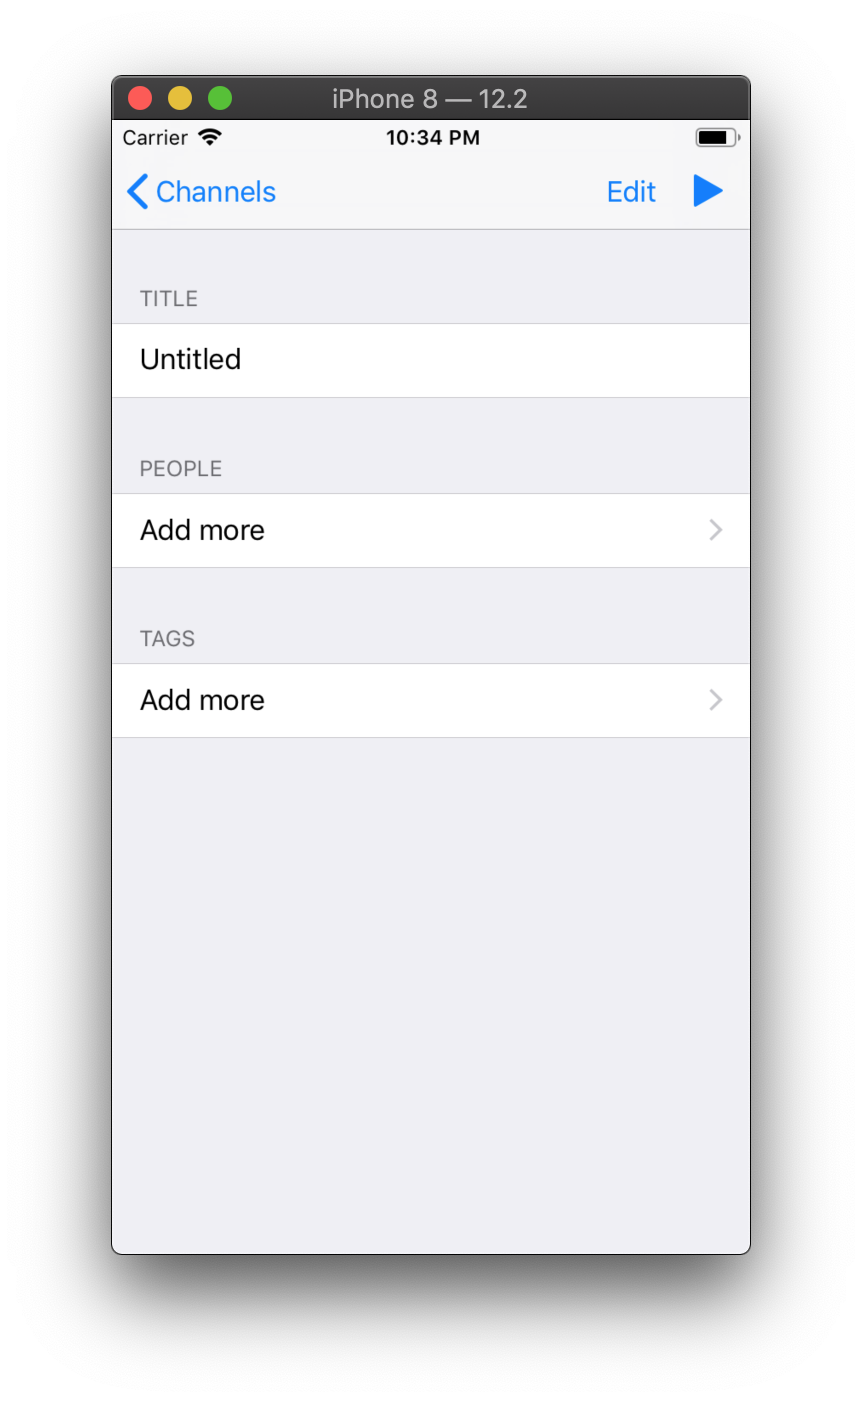
\includegraphics[width=\linewidth]{../includes/pmi/channel_create.png}
		\end{subfigure}
		\begin{subfigure}[b]{0.3\linewidth}
			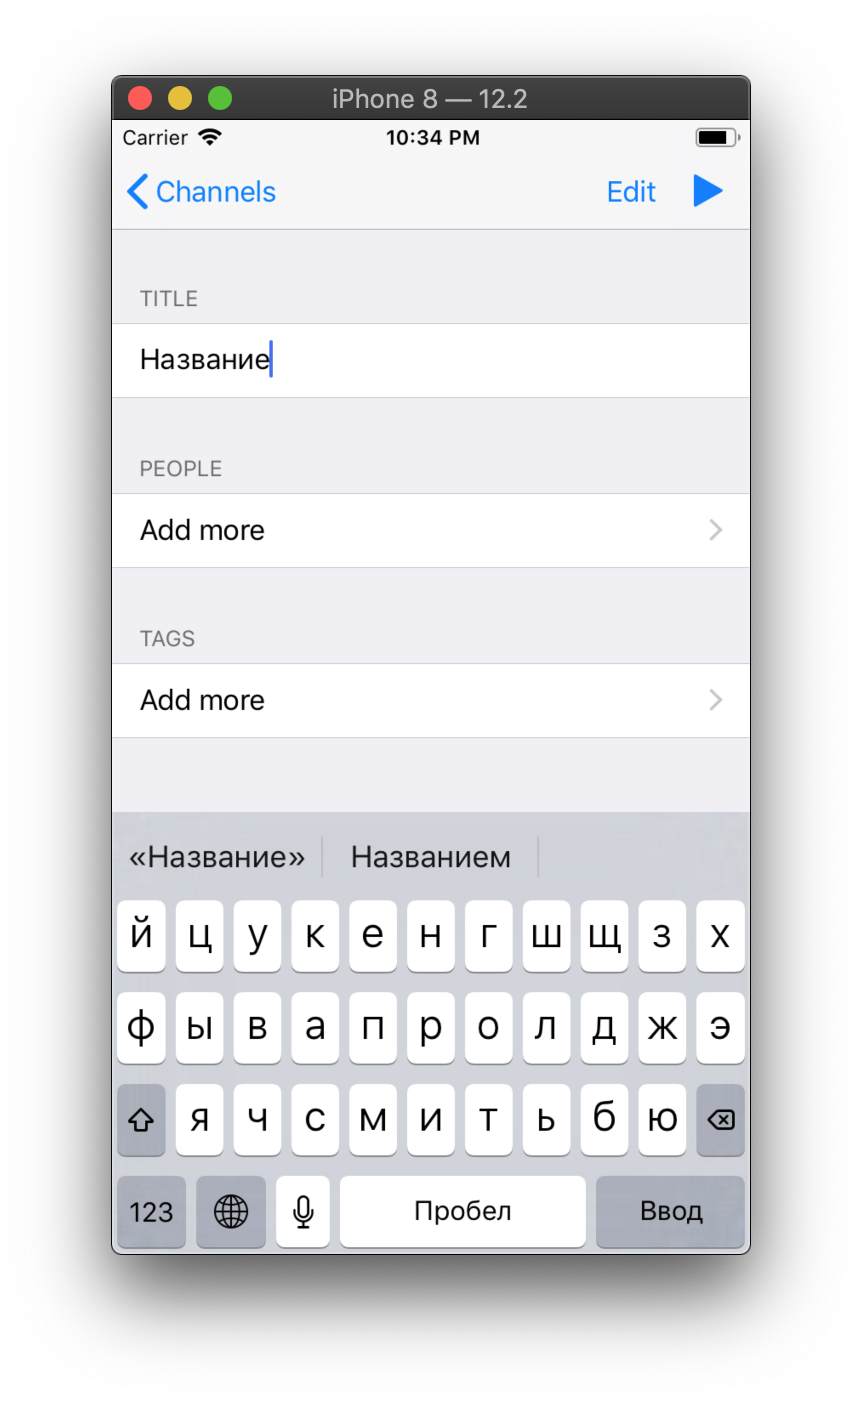
\includegraphics[width=\linewidth]{../includes/pmi/edit_title.png}
		\end{subfigure}
		\caption{Создание канала}
	\end{figure}
	\clearpage

	\paragraph{Редактирование канала\\}
	При  нажатии кнопки \textit{Edit} происходит переход в режим редактирование содержимого канала: по нажатию на красный минус слева от каждой чейки (см. рис \ref{pic: editChannel}) происходит удаление элементов из множества хэштегов и людей. При нажатии ячеек <<Add more>> в зависимости от раздела, в котором находится ячейка, открывается окно для добавления новых людей/хэштегов.
	\begin{figure}[h!]
		\centering
		\begin{subfigure}[b]{0.3\linewidth}
			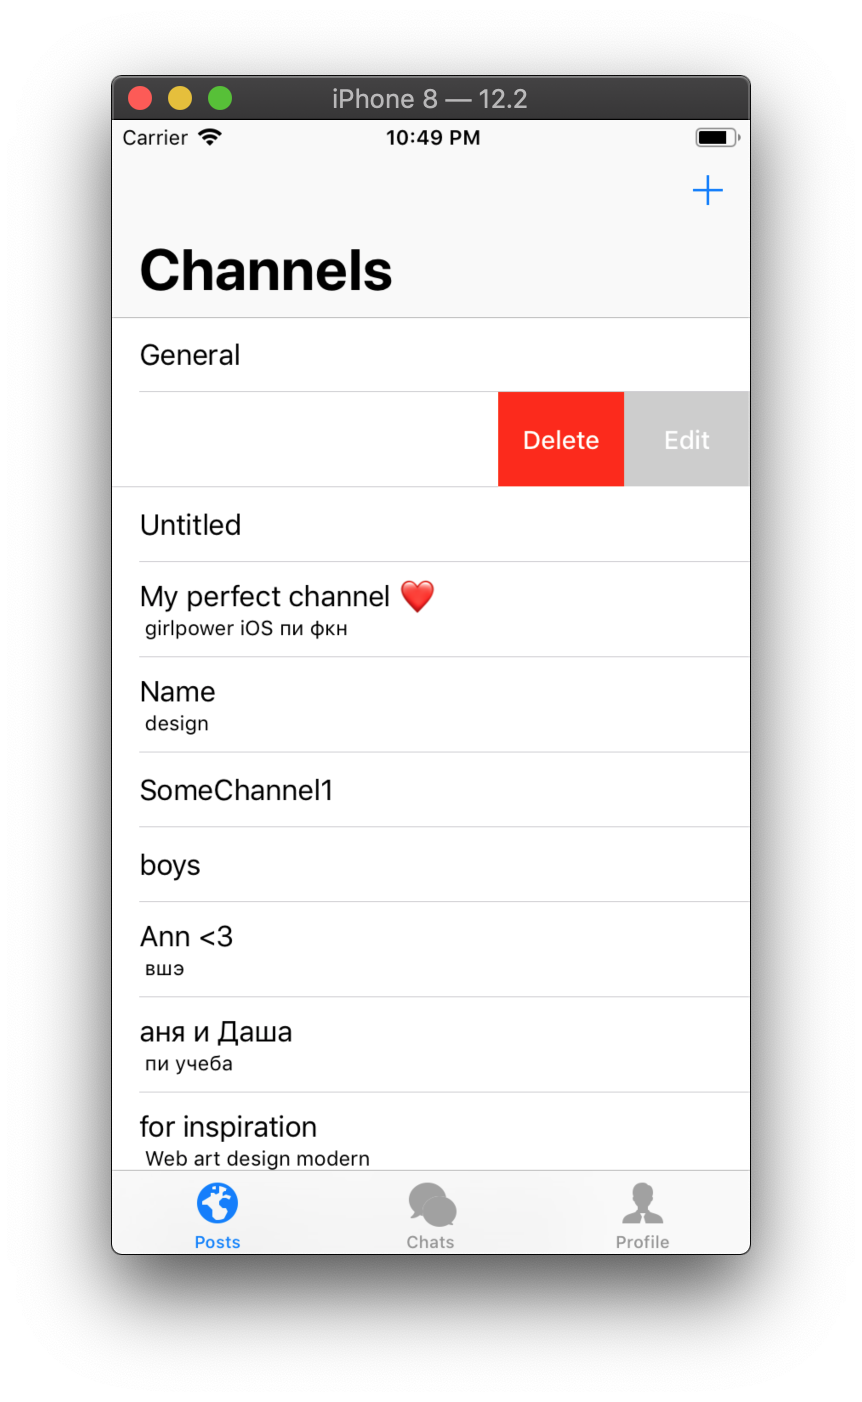
\includegraphics[width=\linewidth]{../includes/pmi/edit.png}
		\end{subfigure}
		\begin{subfigure}[b]{0.3\linewidth}
			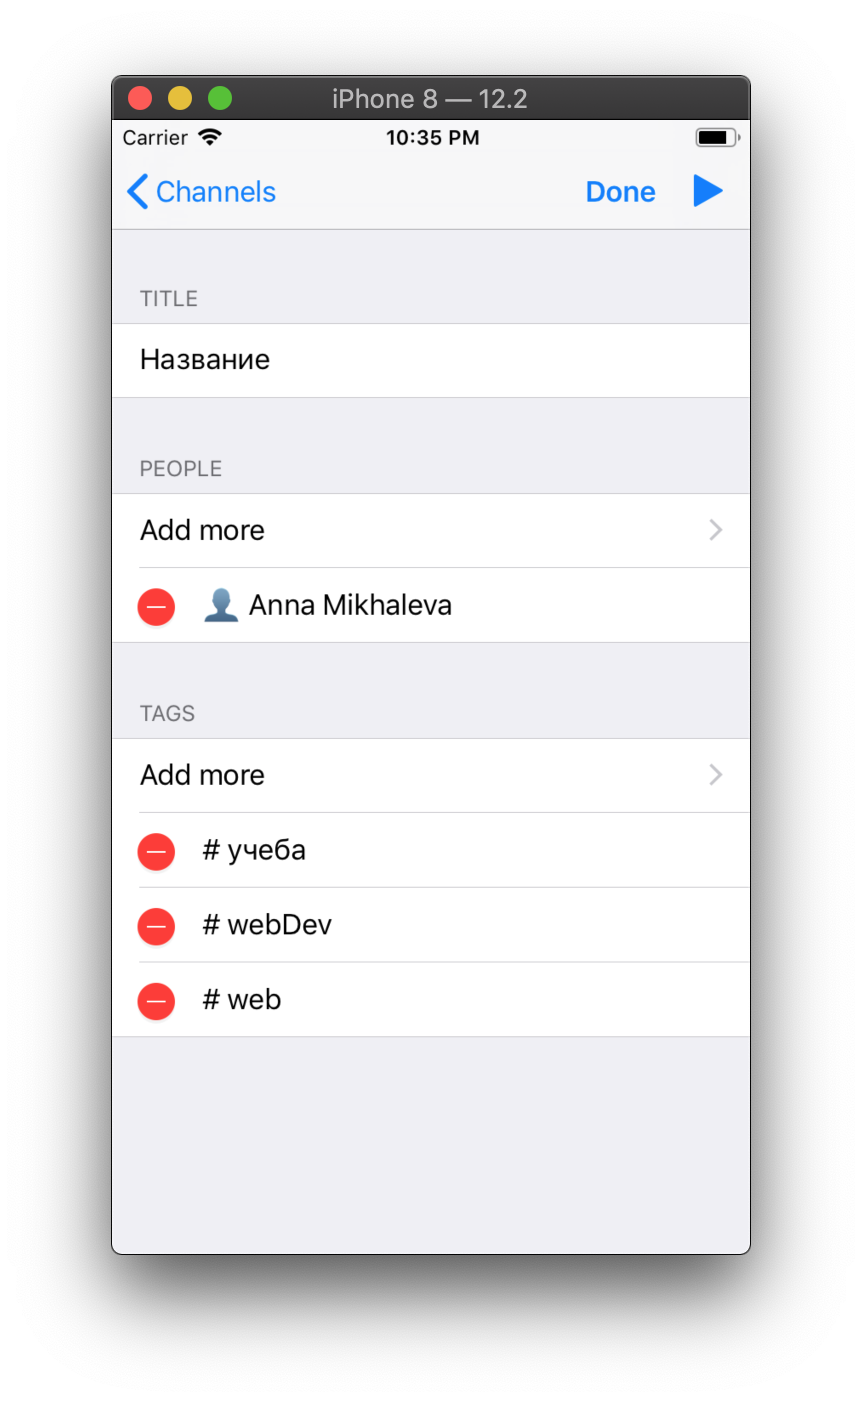
\includegraphics[width=\linewidth]{../includes/pmi/edit_button_channel.png}
		\end{subfigure}
		\begin{subfigure}[b]{0.3\linewidth}
			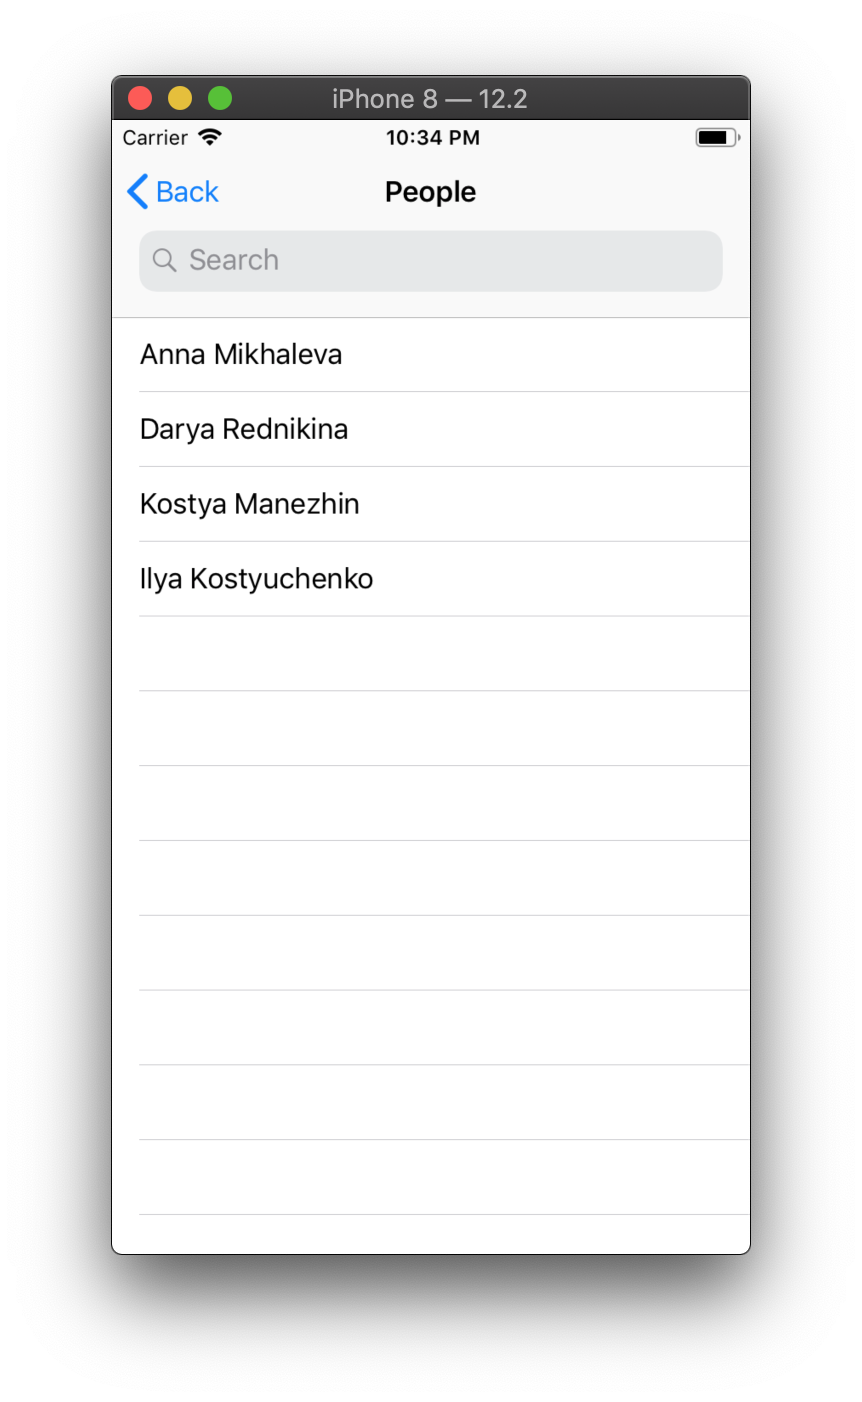
\includegraphics[width=\linewidth]{../includes/pmi/choose_peple.png}
		\end{subfigure}
		\begin{subfigure}[b]{0.3\linewidth}
			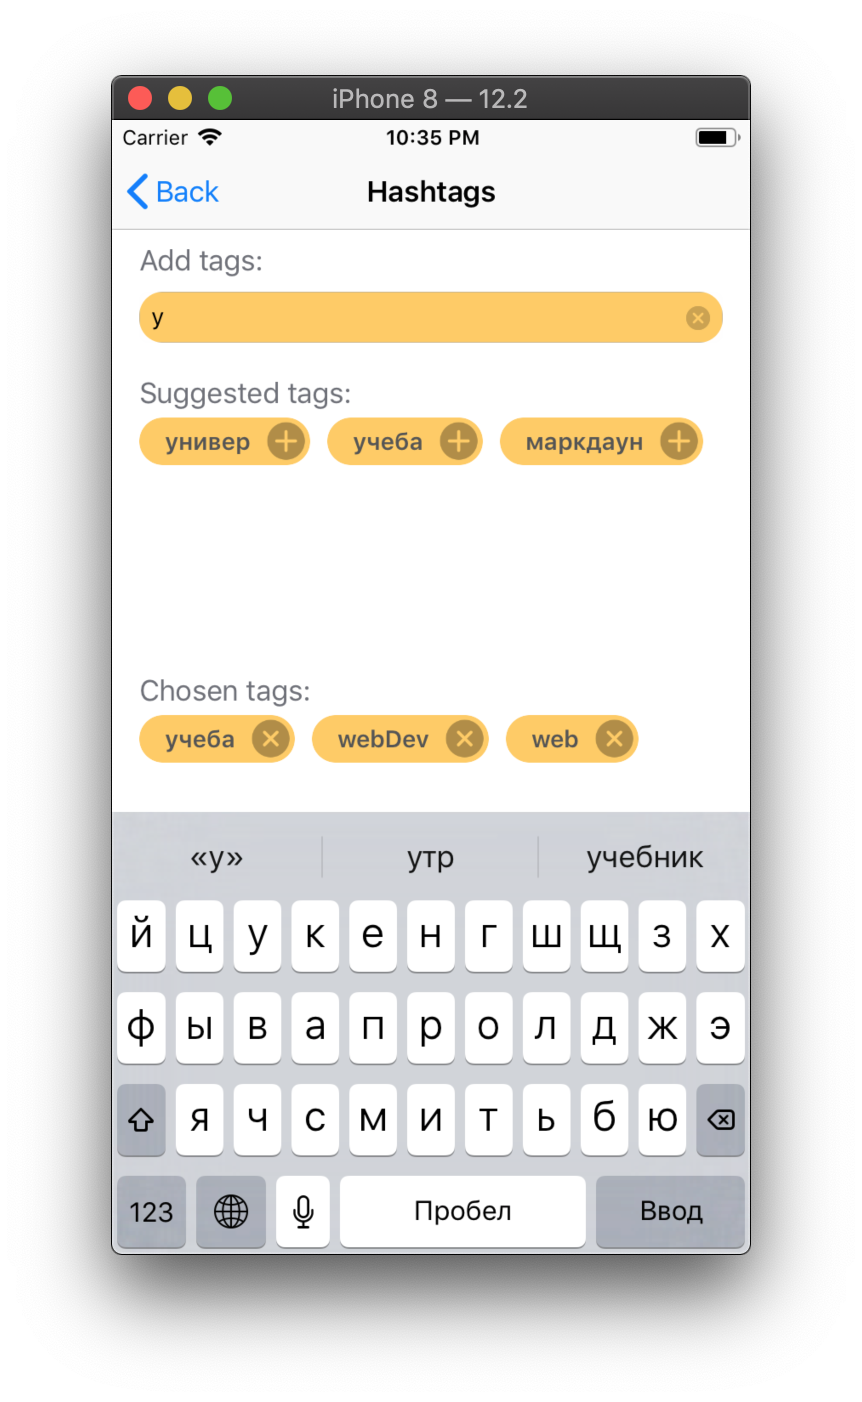
\includegraphics[width=\linewidth]{../includes/pmi/choose_hashtag.png}
		\end{subfigure}
		\begin{subfigure}[b]{0.3\linewidth}
			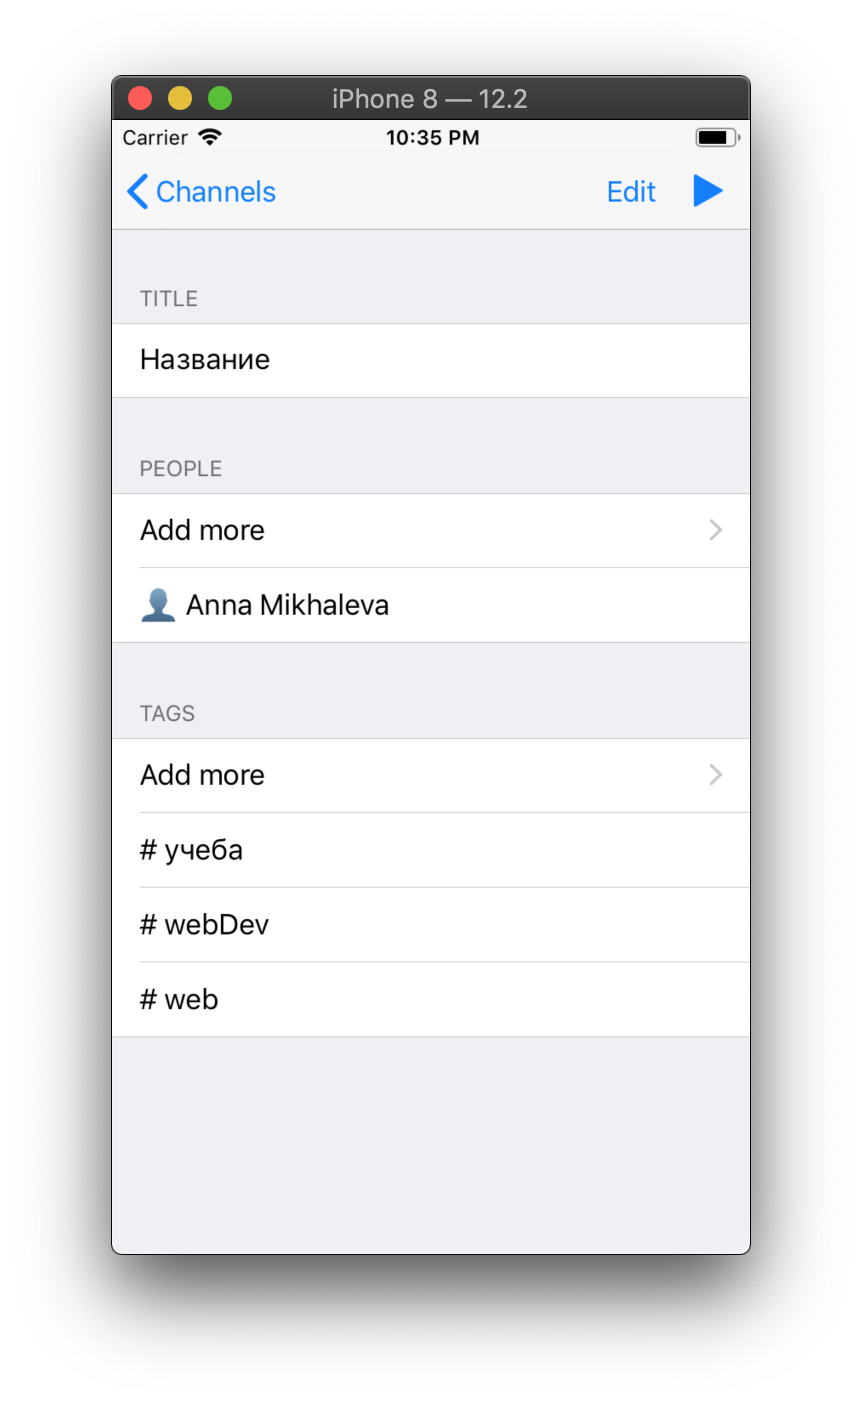
\includegraphics[width=\linewidth]{../includes/pmi/after_editing.png}
		\end{subfigure}
		\caption{\label{pic: editChannel}Редактирование канала}
	\end{figure}
	\clearpage
	\paragraph{Предпросмотр и просмотр содержимого канала\\}
	
	В режиме редактирования переход в режим предпросмотра содержимого канала осуществляется по нажатию на кнопку \textit{Play} в правом верхнем углу экрана. В режиме предпросмотра не доступно нажатие на отображенный пост в ленте для его полного просмотра, а также переход на страницы авторов постов.
	
	Просмотр канала выполняется при нажатии на ячейку с именем канала на экране со списком постов.
	
	\begin{figure}[h!]
		\centering
	\begin{subfigure}[b]{0.3\linewidth}
		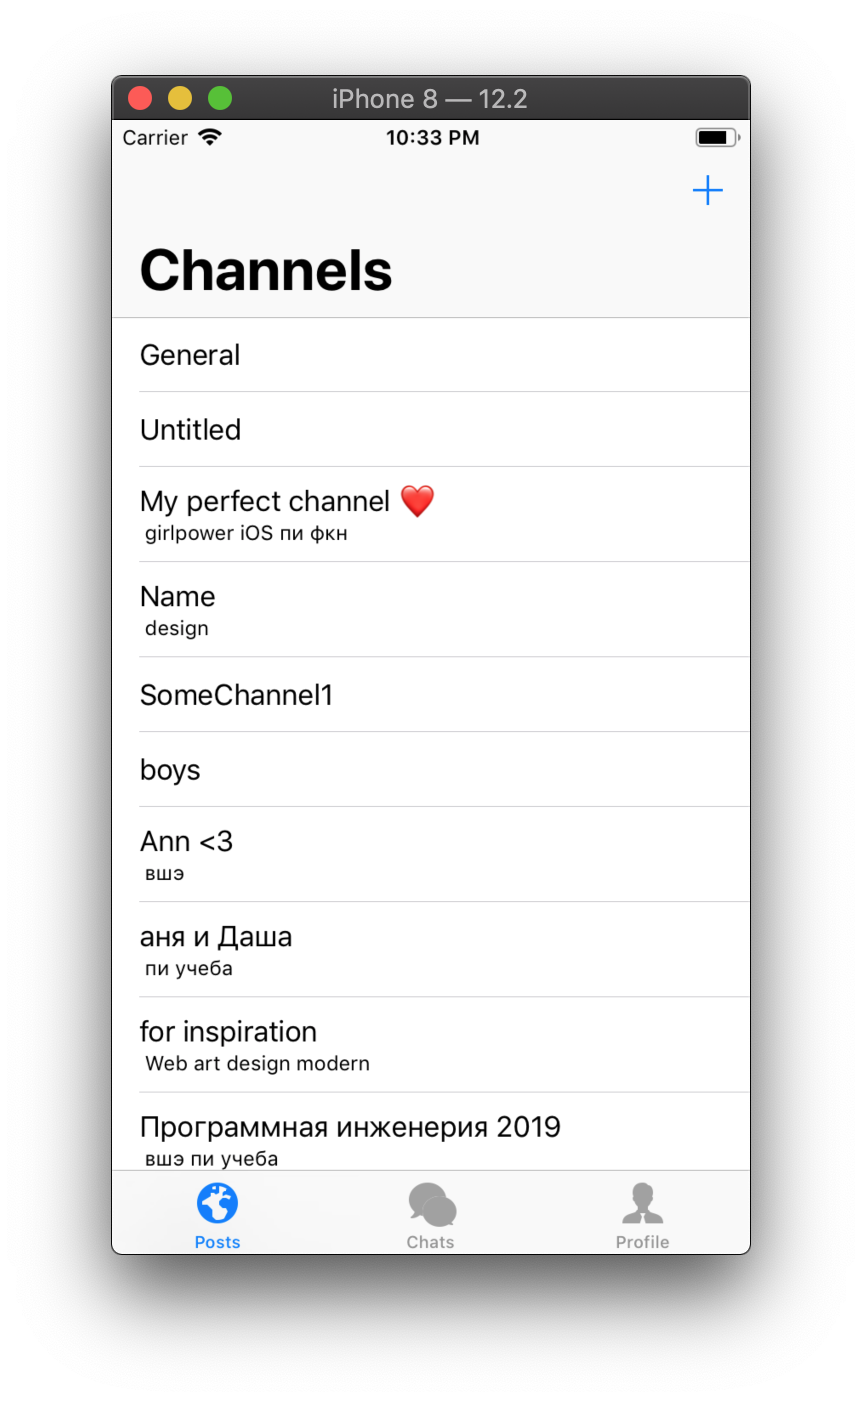
\includegraphics[width=\linewidth]{../includes/pmi/channel_list.png}
	\end{subfigure}
	\begin{subfigure}[b]{0.3\linewidth}
		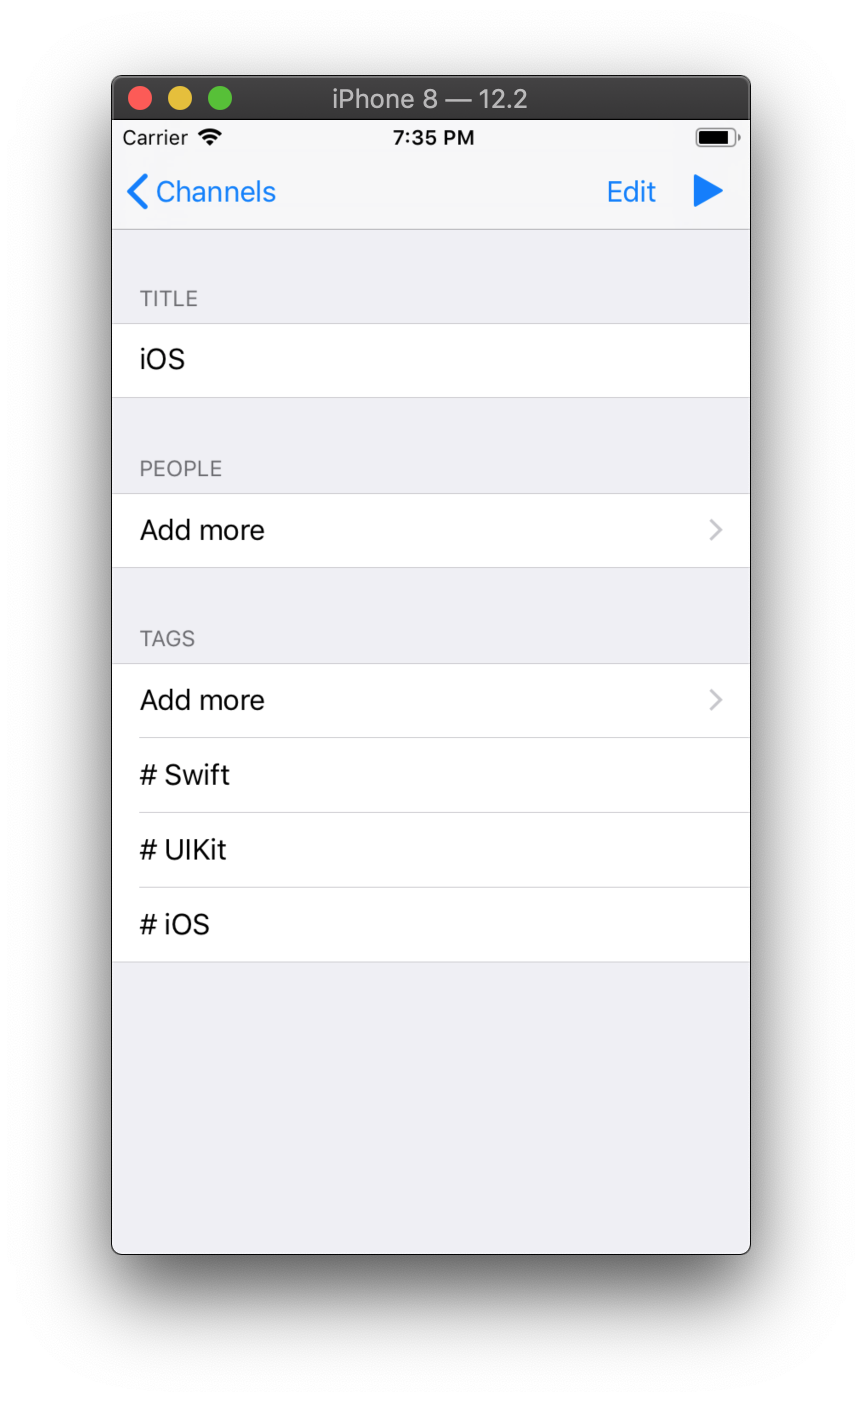
\includegraphics[width=\linewidth]{../includes/pmi/ios_channel_what.png}
	\end{subfigure}
	\begin{subfigure}[b]{0.3\linewidth}
		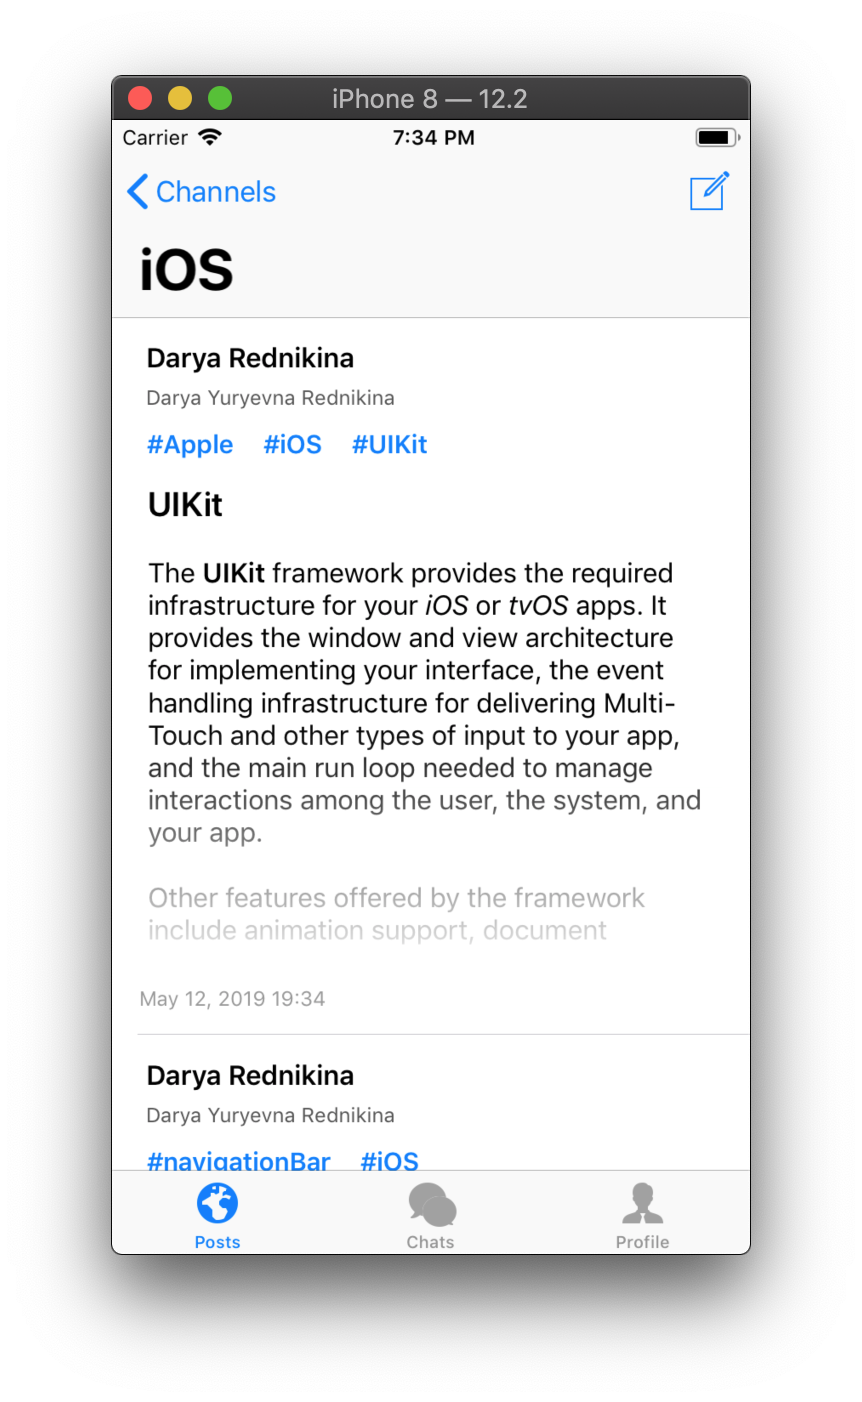
\includegraphics[width=\linewidth]{../includes/pmi/ios_channel.png}
	\end{subfigure}
	\caption{Педпросмотр и просмотр канала}
	\end{figure}
	
	\clearpage 
	\subsubsection{Чаты и беседы: просмотр, создание, редактирование}
	Просмотр списка диалогов доступен при переходе на раздел \textit{Chats} на \textit{tabBar}(\ref{C: tabbar}). При нажатии на ячейку открывается соответственный диалог с сообщениями, написанными ранее. Кнопка \textit{Send} (см. рис. \ref{pic: chats}) предназначена для отправки сообщений. Окно ввода текста для сообщений также поддерживает разметку \textit{markdown}.
		\begin{figure}[h!]
		\centering
		\begin{subfigure}[b]{0.3\linewidth}
			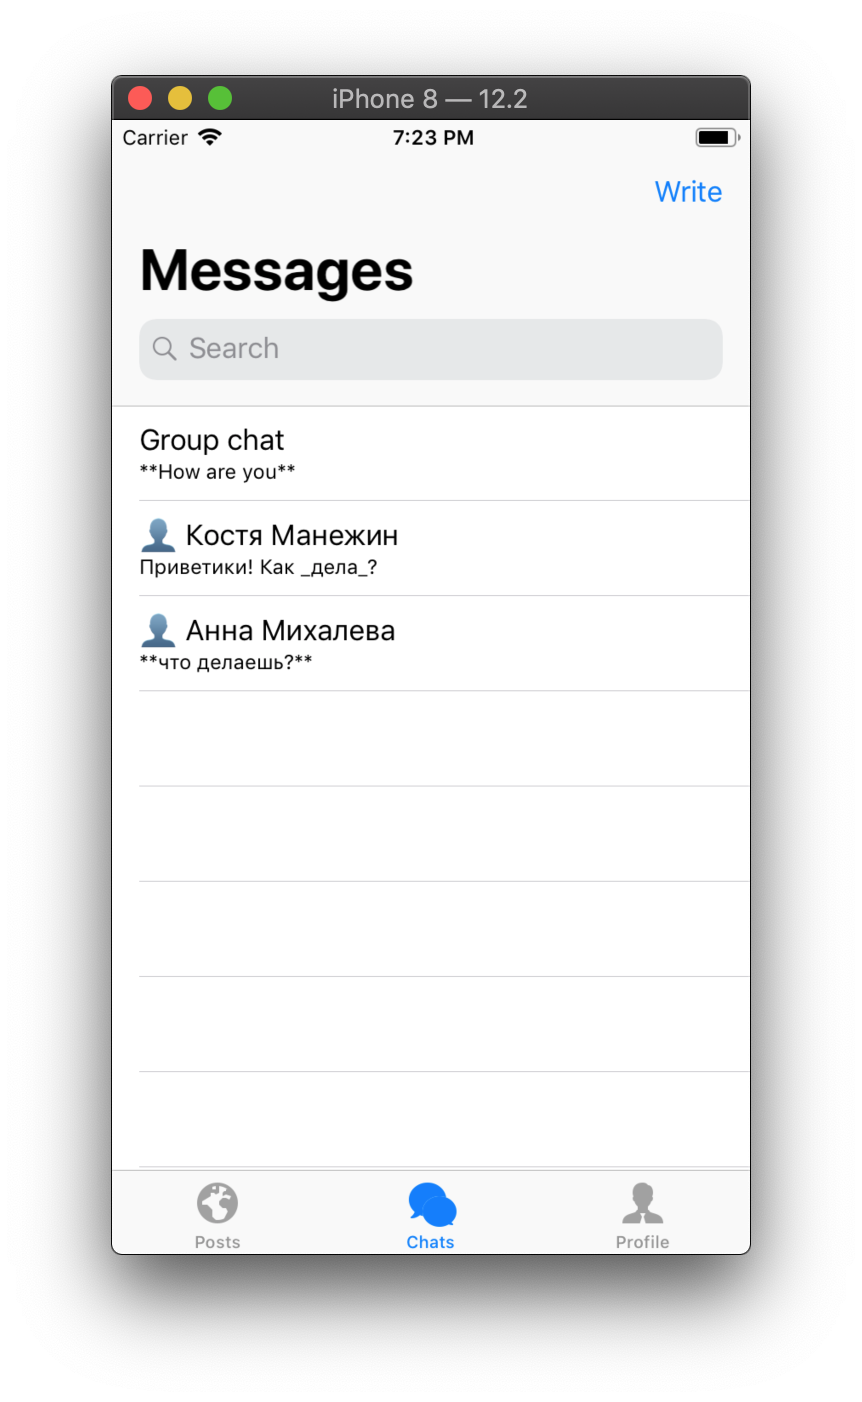
\includegraphics[width=\linewidth]{../includes/pmi/chats.png}
		\end{subfigure}
		\begin{subfigure}[b]{0.3\linewidth}
			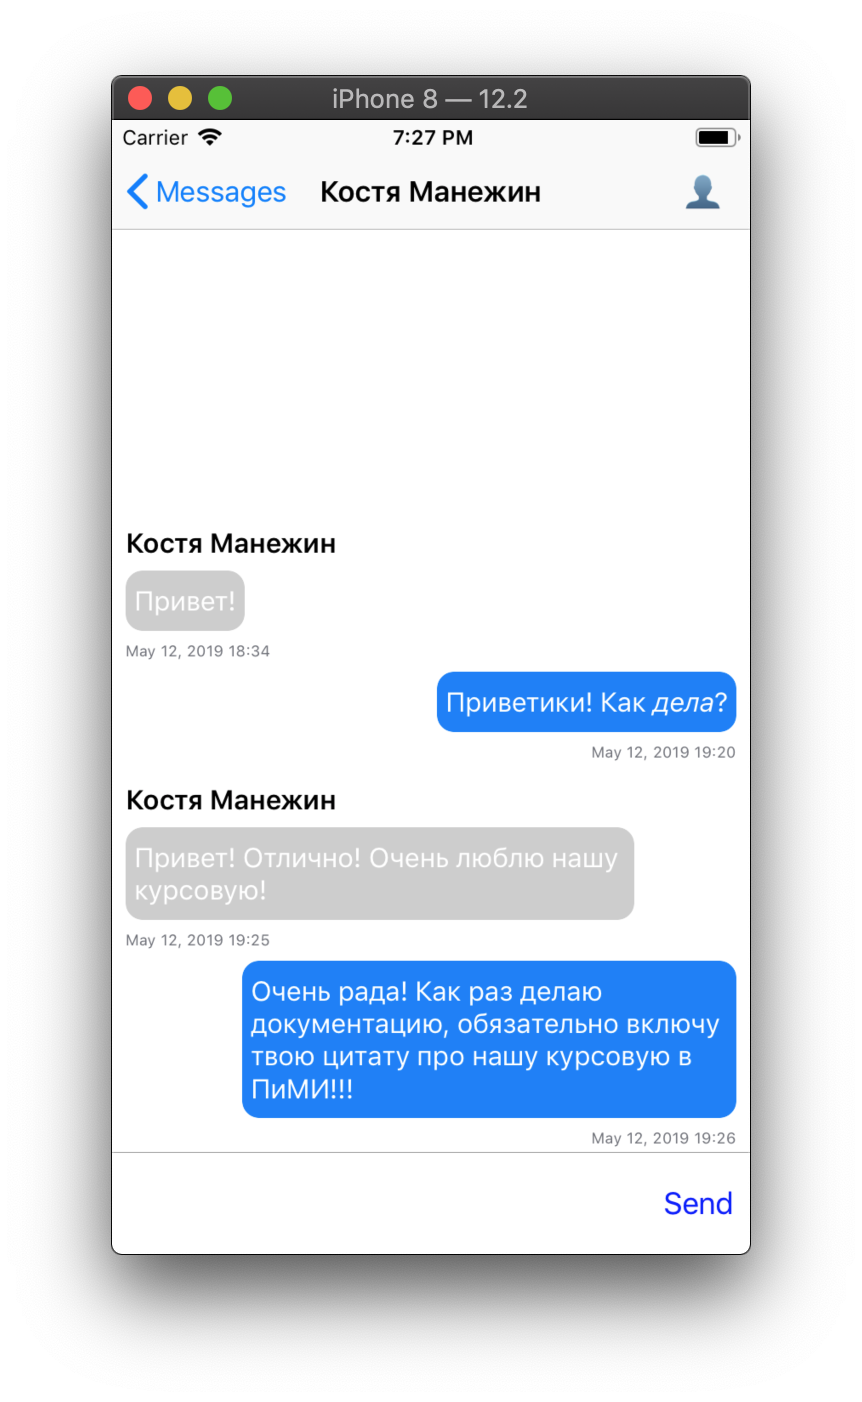
\includegraphics[width=\linewidth]{../includes/pmi/userChat.png}
		\end{subfigure}
		\begin{subfigure}[b]{0.3\linewidth}
			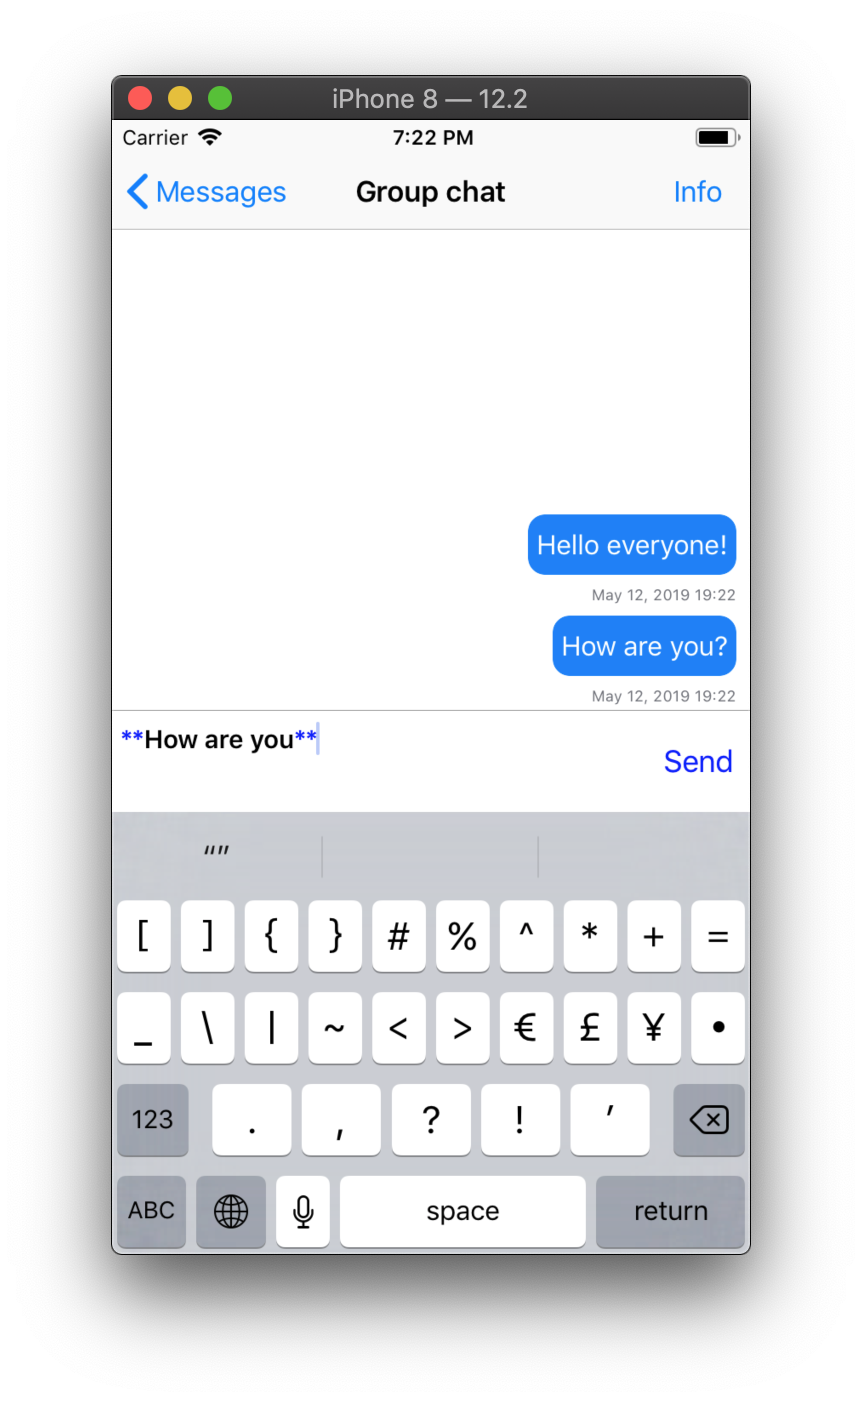
\includegraphics[width=\linewidth]{../includes/pmi/groupChat.png}
		\end{subfigure}
		\caption{\label{pic: chats}Беседы и чаты}
	\end{figure}
	Права администратора беседы имеет либо создатель беседы, либо любой из участников беседы, назначенный другим администратором (см. рис. \ref{pic: admin}). Также администратор может поменять название беседы и состав участников по нажатию на соответствующие ячейки в секции \textit{Title} и  \textit{Participants} (см. рис. \ref{pic: admin}). Также выйти из чата можно с помощью нажатия на кнопку \textit{Leave chat}.
	\begin{figure}[h!]
		\centering
		\begin{subfigure}[b]{0.3\linewidth}
			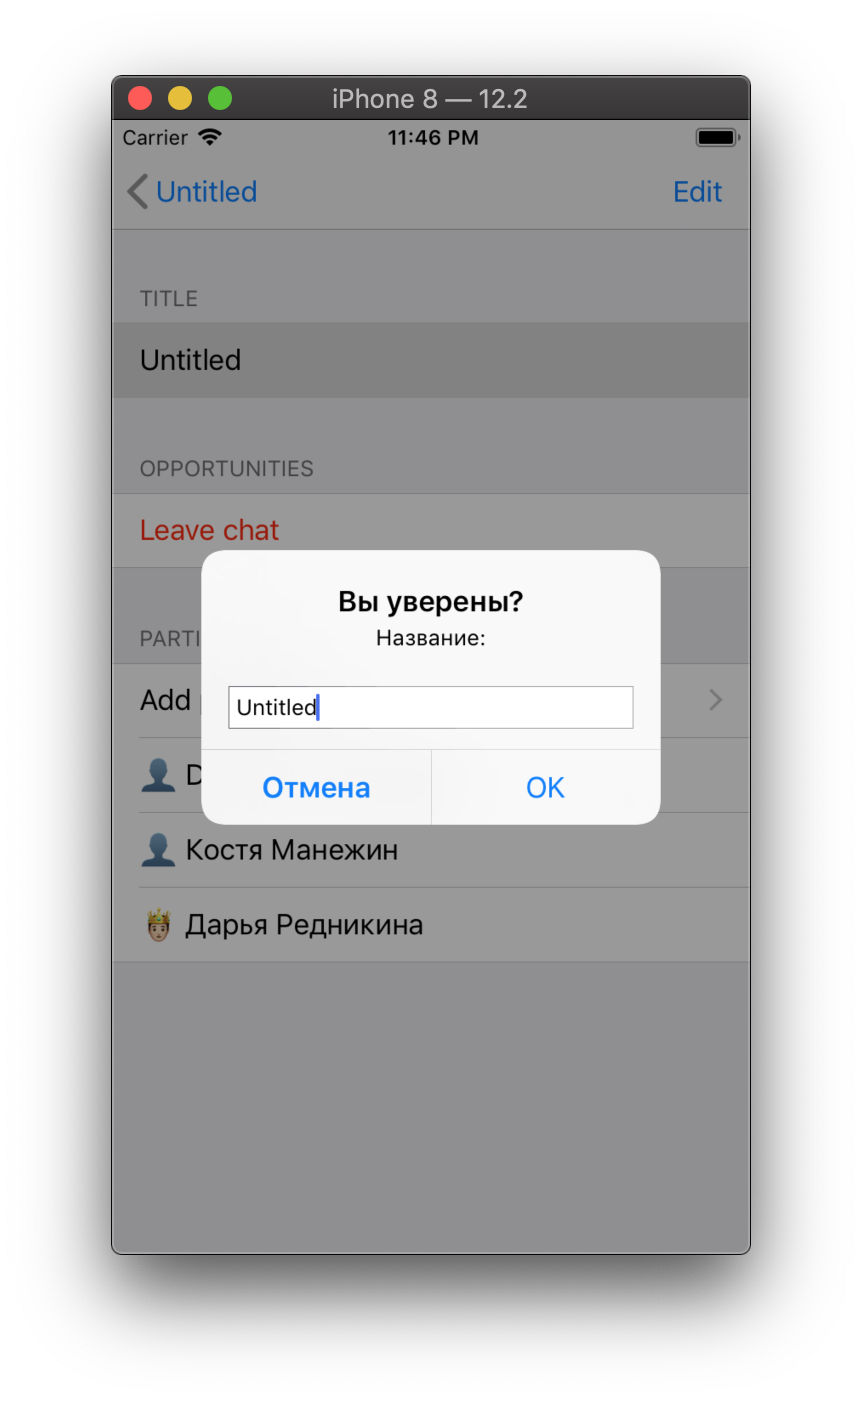
\includegraphics[width=\linewidth]{../includes/pmi/adminName.png}
		\end{subfigure}
		\begin{subfigure}[b]{0.3\linewidth}
			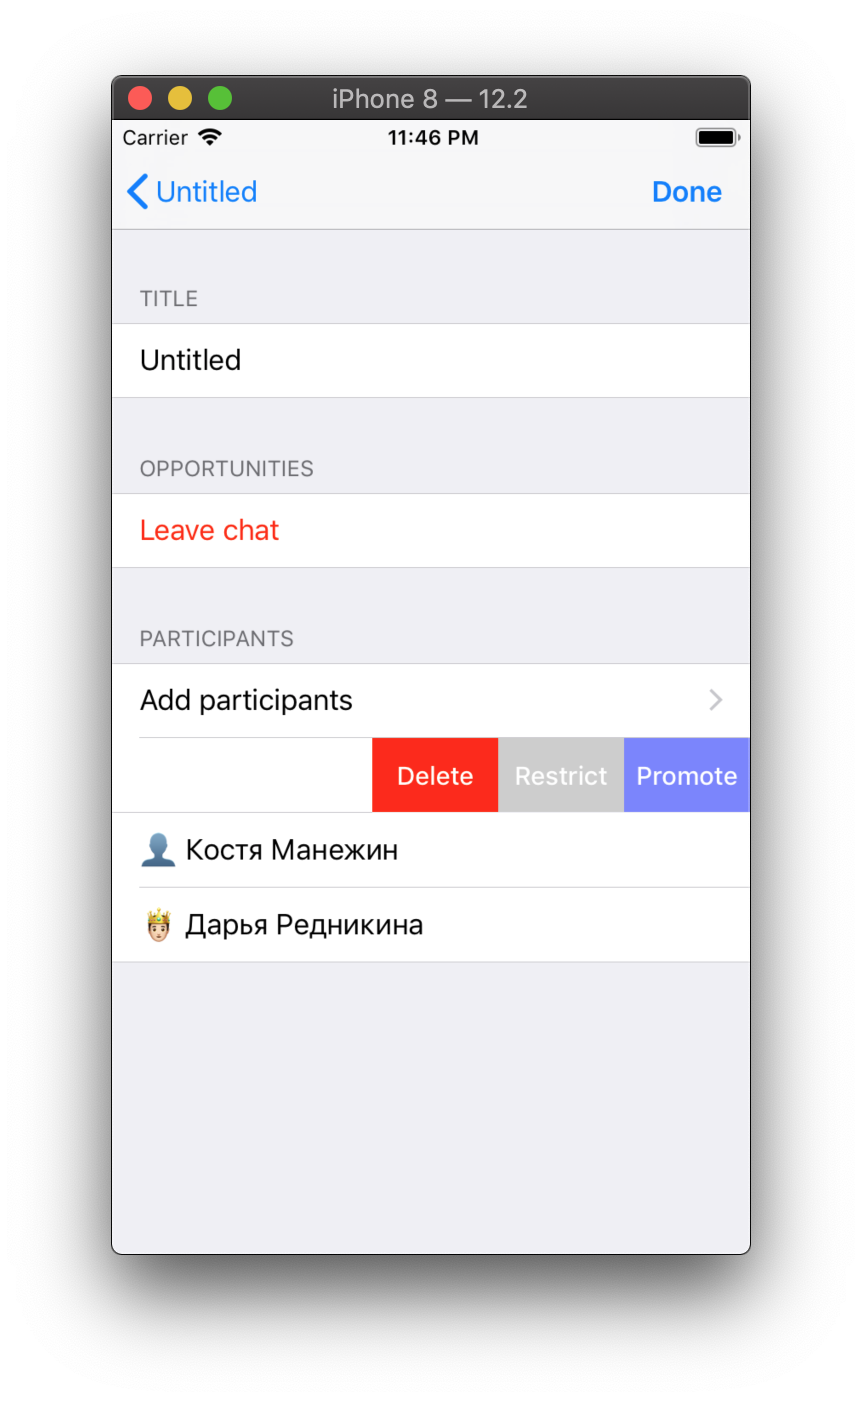
\includegraphics[width=\linewidth]{../includes/pmi/adminChange.png}
		\end{subfigure}
		\caption{\label{pic: admin}Администрирование беседы}
	\end{figure}
	\subsection{Проверка требований к надежности}
	 В процессе выполнения всех остальных испытаний программа продолжала функционировать без перебоев со стороны приложения.
	\subsection{Проверка требований к программной документации}
	Вся документация, представленная в требованиях, готова.
	
						\newpage
	\patchcmd{\thebibliography}{\section*{\refname}}{}{}{}
	\addition{Список источников}
	\begin{thebibliography}{6}
		\bibitem{interface} Human Interdace Guidelines [Электронный ресурс] URL: \url{https://developer.apple.com/design/human-interface-guidelines/ios/overview/themes} (Дата обращения: 16.05.2019, режим доступа: свободный)
		\bibitem{UIKit} UIKit [Электронный ресурс] URL: \url{https://developer.apple.com/documentation/uikit} (Дата обращения: 16.05.2019, режим доступа: свободный)
		\bibitem{gost}Единая система программной документации – М.: ИПК, Издательство стандартов, 2000, 125 стр.
		\bibitem{terms} Terms of use for Apple products [Электронный ресурс] URL: \url{https://www.apple.com/legal} (Дата обращения: 16.05.2019, режим доступа: свободный)
		\bibitem{lms} 
		LMS [Электронный ресурс] URL: 
		\url{https://lms.hse.ru} (Дата обращения: 16.05.2019, режим доступа: свободный)
		\bibitem{server} GitHub repository ilyakoo0/denis [Электронный ресурс] URL: \url{https://github.com/ilyakooo0/denis} (Дата обращения: 16.05.2019, режим доступа: свободный)
		\bibitem{threads} 
		How to design social media interactions 
		[Электронный ресурс] URL:
		\url{https://medium.com/@michaelchaika/ho-to-design-social-media-interactions-386bdb5bee6d} (Дата обращения: 16.05.2019, режим доступа: свободный)
	\end{thebibliography}

	\addition{Иллюстрации интерфейса} \label{interface}
	\begin{figure}[h!]
		\centering
		\begin{subfigure}[b]{0.3\linewidth}
			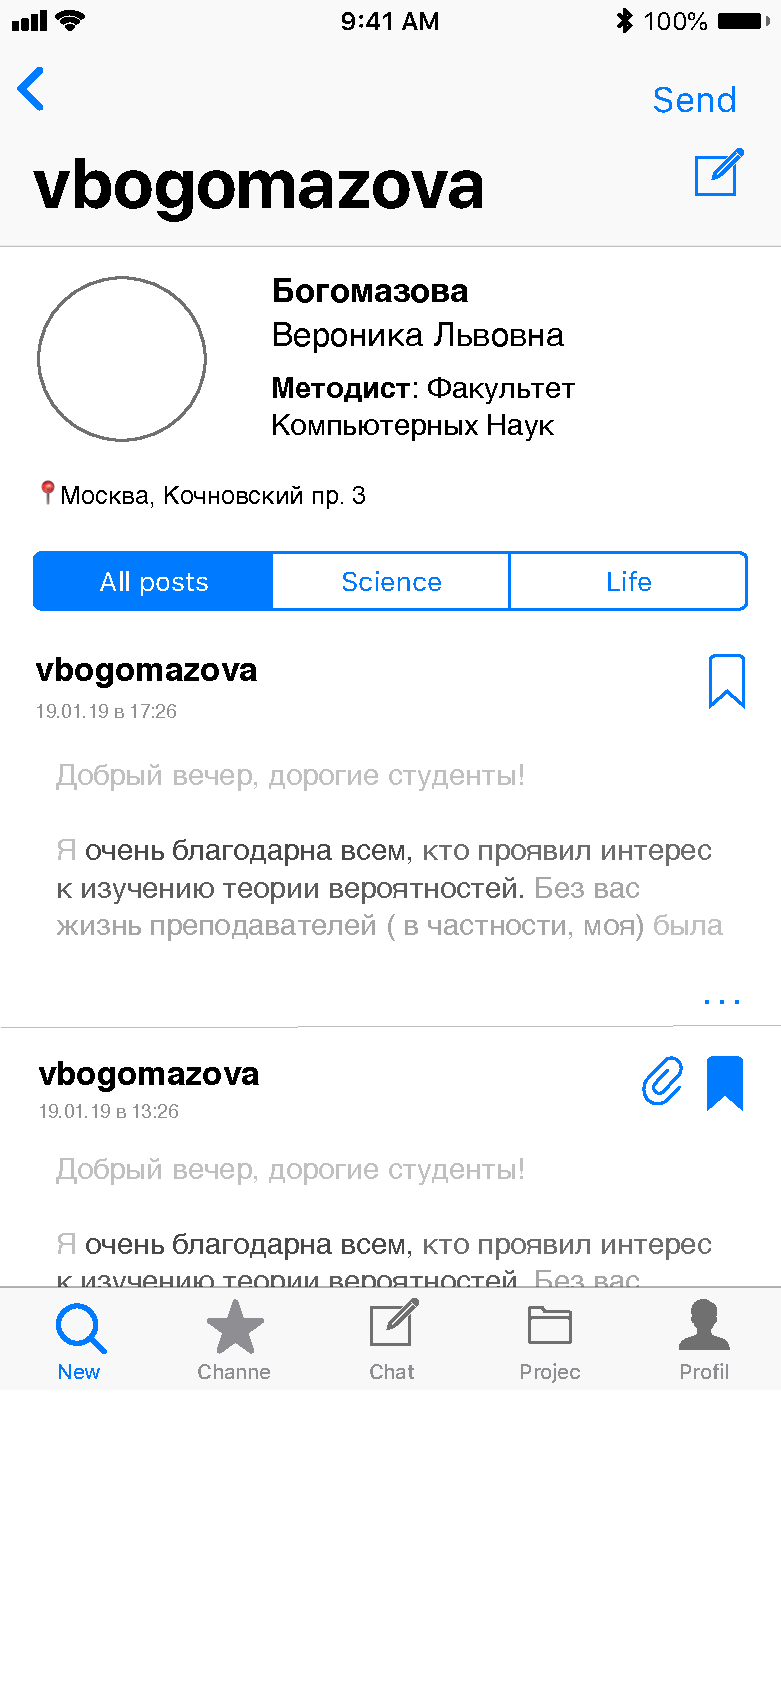
\includegraphics[width=\linewidth]{../includes/prototype/1.pdf}
		\end{subfigure}
		\begin{subfigure}[b]{0.3\linewidth}
			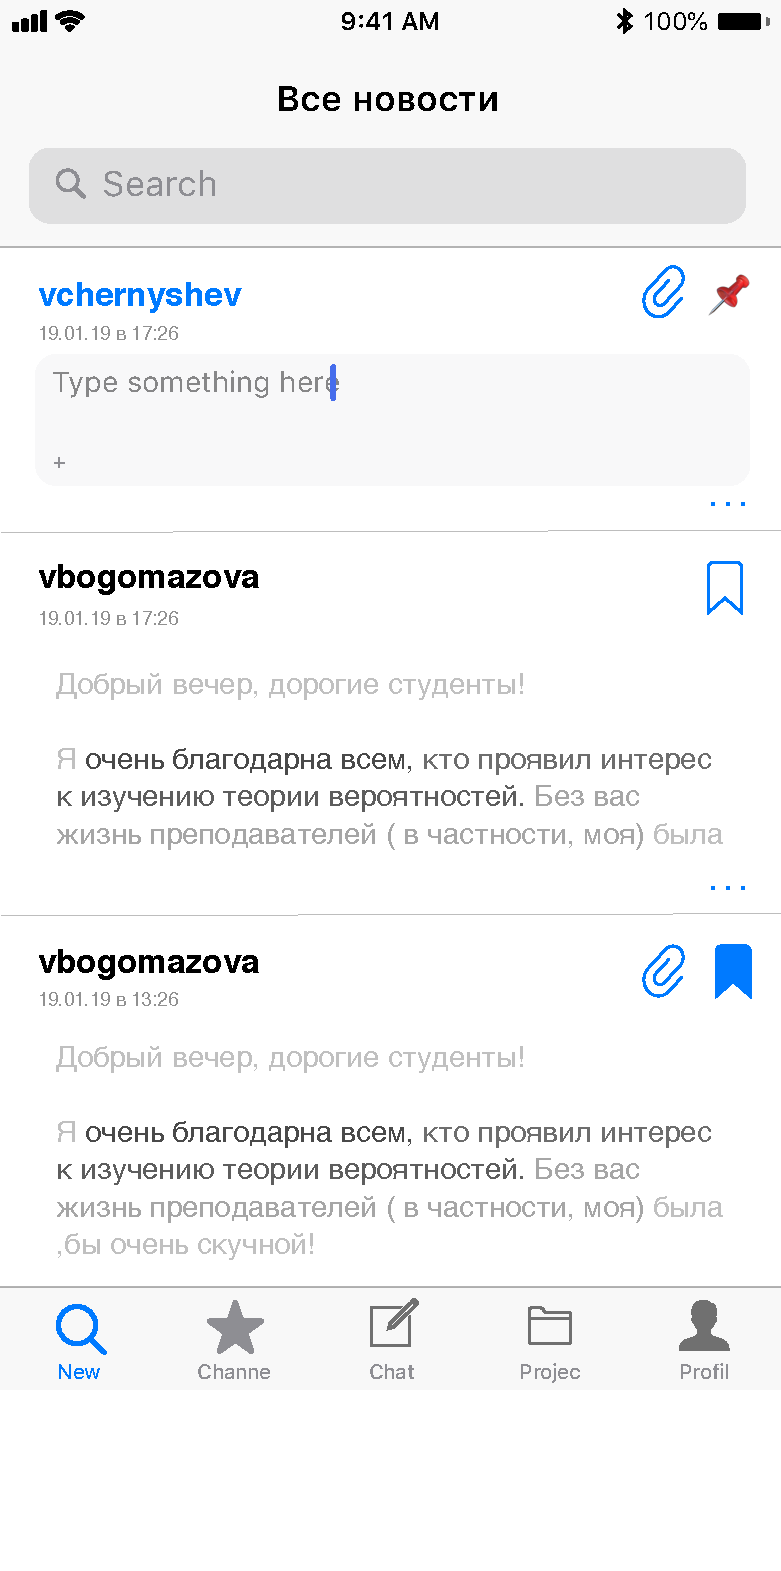
\includegraphics[width=\linewidth]{../includes/prototype/2.pdf}
		\end{subfigure}
		\begin{subfigure}[b]{0.3\linewidth}
			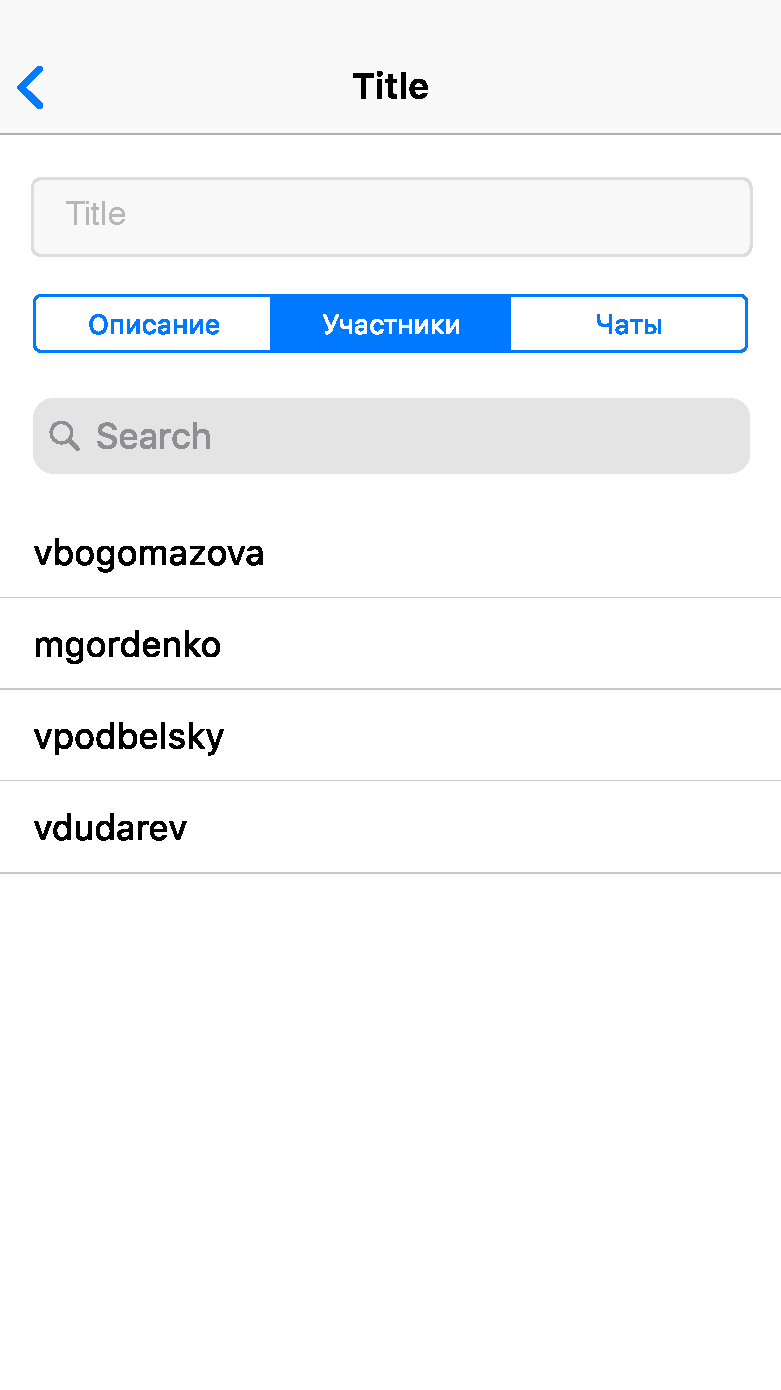
\includegraphics[width=\linewidth]{../includes/prototype/6.pdf}
		\end{subfigure}
		\begin{subfigure}[b]{0.3\linewidth}
			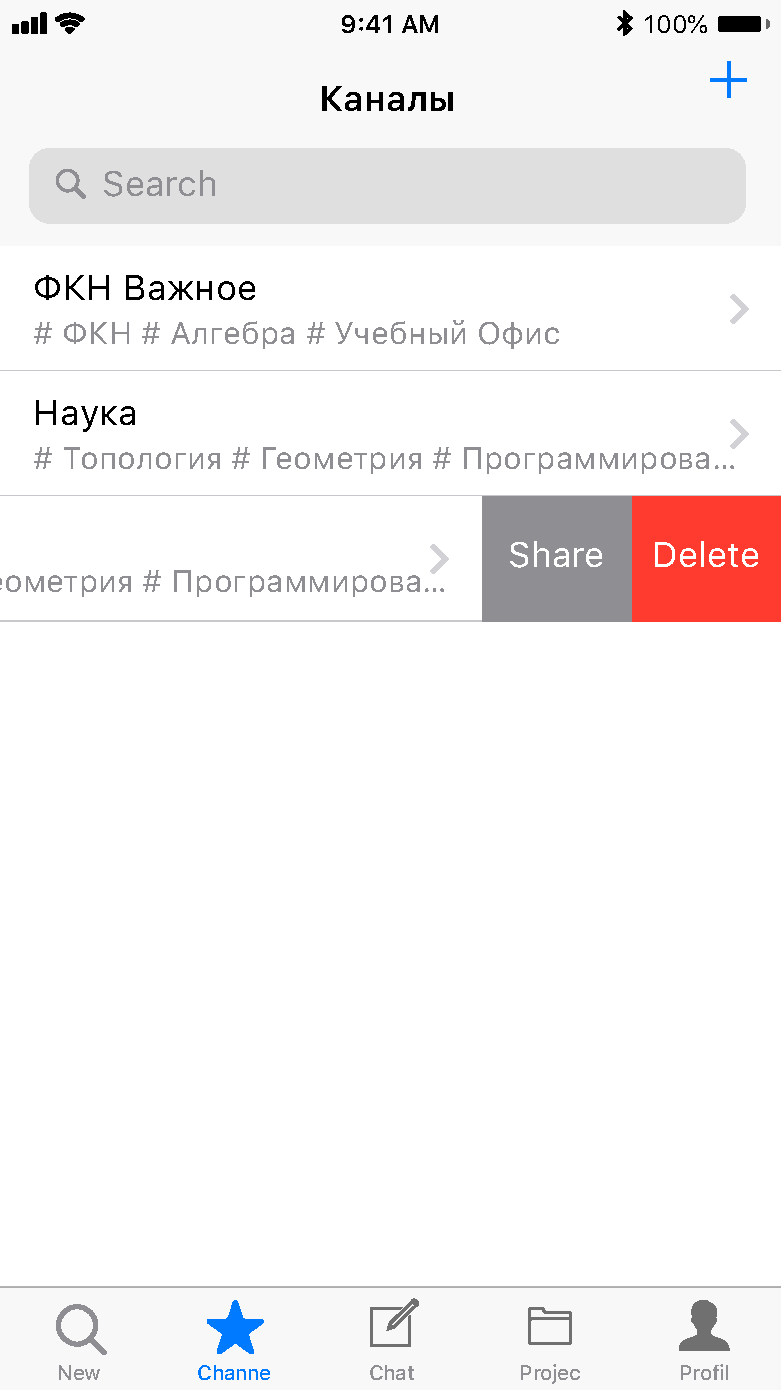
\includegraphics[width=\linewidth]{../includes/prototype/4.pdf}
		\end{subfigure}
		\begin{subfigure}[b]{0.3\linewidth}
			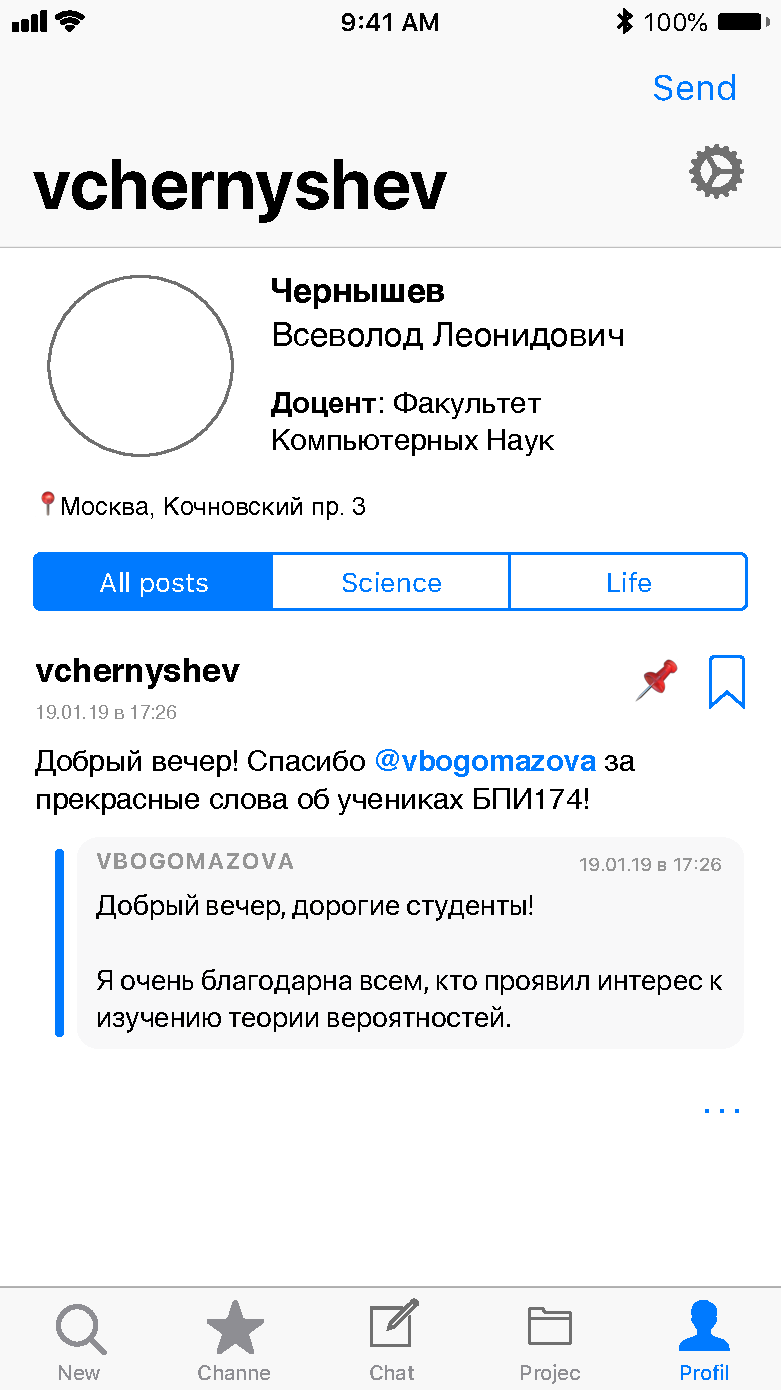
\includegraphics[width=\linewidth]{../includes/prototype/5.pdf}
		\end{subfigure}
		\begin{subfigure}[b]{0.3\linewidth}
			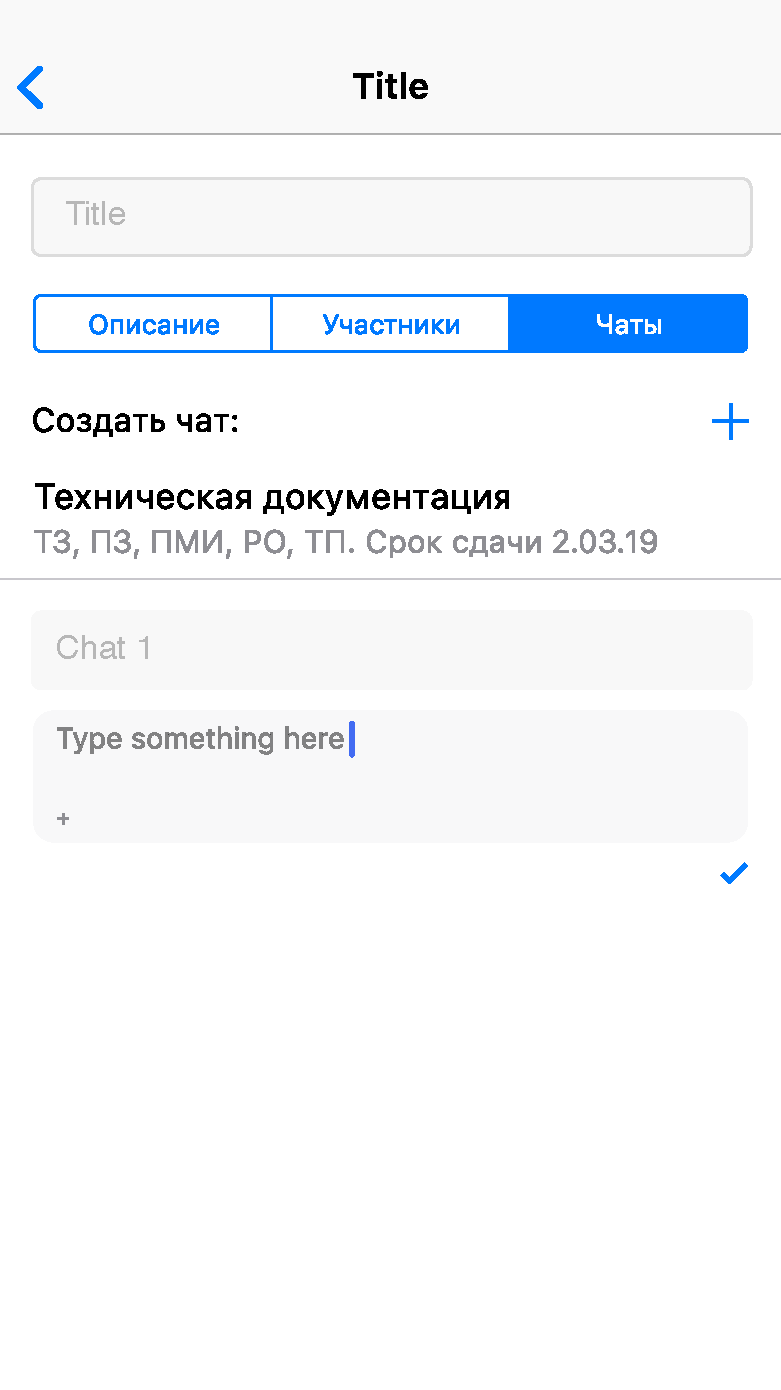
\includegraphics[width=\linewidth]{../includes/prototype/8.pdf}
		\end{subfigure}
		\caption{Прототип интерфейса}
	\end{figure}


	\addition{Используемые понятия и определения} 
	\begin{description}
		\item[Социальная сеть] -- это интернет-площадка, сайт, который позволяет зарегистрированным на нем пользователям размещать информацию о себе и коммуницировать между собой, устанавливая социальные связи
		\item[Хэштег] -- ключевое слово или несколько слов сообщения, тег (пометка), используемый в микроблогах и социальных сетях, облегчающий поиск сообщений по теме или содержанию и начинающийся со знака решётки \label{term: hash}
		\item[Пост] -- информационный блок, размещённый пользователем в социальной сети на своей странице и содержащий набор хэштегов, по которым его можно найти \label{term: post}
		\item[Канал] -- сохраненные ранее созданные фильтры новостей (набор хэштегов) по всем публичным постам \label{term: channel}
		\item [Беседа] -- чат для пользователей, в котором одновременно могут присутствовать от 3 до 50 участников \label{term: chat}
		\item [Проект]  -- раздел, в котором сотрудники с любых факультетов по приглашению смогут вместе работать над каким-либо научным исследованием. Проект состоит из timeline (лента с новостями для всех участников проекта) и набором чатов и бесед (с разным количеством участников в каждой) \label{term: project}
		\item [Preview канала]  -- предпросмотр ленты канала с ограничениями на просмотр полной версии поста в ленте, переходом на страницы авторов, нажатия на хэштеги \label{term: preview}
		\item [Preview поста]  -- ограниченный контент (содержание) поста в ленте \label{term: previewPost}
		\item [Action sheet] это особый стиль оповещения, который появляется в ответ на элемент управления или действие и представляет собой набор из двух или более вариантов выбора, связанных с текущим контекстом. \label{C: actionSheet}
		\item [TabBar] в дизайне - интерфейс документа с вкладками или вкладка, представляющая  собой графический элемент управления, который позволяет нескольким документам или панелям содержаться в одном окне, используя вкладки в качестве навигационные виджеты для переключения. \label{C: tabbar}
	\end{description}
	
	\addition{Статус требований}
	\begin{longtable}{|p{0.2\linewidth}|p{0.5\linewidth}|} 
	\caption{Статус требований} \label{statusReq} \\
\hline
\textbf{Proposed} & Требование запрошено авторизированным источником \\ \hline
\textbf{Approved} & Требование проанализировано, его влияние на проект просчитано, и оно было размещено в базовой версии определенной версии. \\ \hline
\textbf{Implemented} & Код, реализующий требование, разработан, написан и протестирован. Требование отслежено до соответствующих элементов дизайна и кода \\ \hline
\textbf{Verified} & Корректное функционирование реализованного требования подтверждено в соответствующем продукте. Требование отслежено до соответствующих вариантов тестирования. Теперь требование считается завершенным \\ \hline
\textbf{Deleted} & Утвержденное требование удалено из базовой версии.  \\ \hline
\textbf{Rejected} & Требование предложено, но не запланировано для реализации ни в одной будущих версий. \\ \hline

\end{longtable}

	
	\listRegistration
	%\addcontentsline{toc}{section}{Лист регистрации изменений}
\end{document} % конец документа